\documentclass[../report.tex]{subfiles}
\begin{document}
\chapter{Literature Study}
\label{ch:literature_study}

\newfontfamily\myfont{Times new roman}

The thesis project commences with a study of literature, this is intended to introduce the main concepts that will be used as the foundation of the methodologies used, as well as supplement the discussion of any results gathered. Literature studies are conducted in fields related to the research project, thus the first field to be surveyed will be that of Reinforcement Learning, and the second field to be surveyed is the developments of the Flying-V. 

The sections on adp and drl will start with touching on the earlier examples of algorithms, and moving progressively to touching on the respective state of the art.

\section{Reinforcement Learning Foundations}

The basic idea of reinforcement learning is to have some agent associate rewards with actions that help realize a goal and promote the agent to take more of such actions by asking it to maximize the reward. The agent is not told what the goal is explicitly, its' only interface with the world around it is through executing these actions, and observing that it has transitioned into some state and received some reward. Reinforcement learning can be thought of as a way in which theorists have attempted to codify and formulate algorithms for, the universal experience of learning through trial and error. Much like how a child learns to walk, or a dog learns to sit, it is through reinforcement learning that machines can learn how to perform tasks that might not be easily programmed. Through this codification, computer programs have been made that demonstrated impressive levels of learning; for example, programs can learn through reinforcement learning to play various high-dimensional board games to a level of expertise surpassing any living player \cite{alpha_zero}, and a robotic arm can learn hand dexterity and mimic the hand movements of a human \cite{OpenAI_dexterity}.

Understanding how the reinforcement learning algorithms work behind such examples and how they may be applied to flight control will require understanding the foundations first, thus this section will introduce the basic terminologies and ideas used to build these algorithms.


\subsection{Markov Decision Process}

The \ac{mdp} is the mathematical framework that is used to model sequential decision processes such as how an agent interacts with an environment, and it is what contextualizes all the ideas in reinforcement learning, for instance, the basic notion that an agent performs an action and receives a reward.

In such a framework, there exist two entities: the agent and the environment, and information flows from one entity to another to model making decisions and their resulting consequences. In reinforcement learning the agent is sometimes also called the learner, it selects an action $A_t$ which gets fed to the environment, and the environment will provide the corresponding state $S_{t+1}$ which the agent has transitioned to as a result of action $A_t$ and the reward associated to that state transition $R_{t+1}$, the agent can subsequently use $S_{t+1}$ and $R_{t+1}$ to decide on the next time step's action $A_{t+1}$. A graphical depiction of this agent-environment interface in the \ac{mdp} is shown in \autoref{fig:mdp}.

\begin{figure}[H]
    \centering
    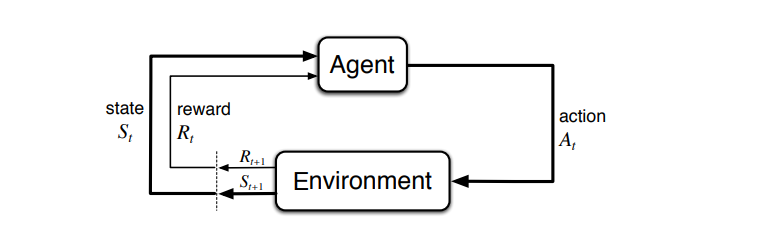
\includegraphics[width=\textwidth]{figures/01/mdp.png}
    \caption{Flow diagram of the agent-environment interaction central to the \ac{mdp}}
    \label{fig:mdp}
\end{figure}

This time trace of an agent-environment interaction is recorded in a so-called \textit{trajectory} $\mathcal{T}$, which is a chain of state-action-reward-next state values for the entire duration of the decision process:

\begin{equation} \label{eq:trajectory}
    \mathcal{T} = S_{0}, A_{0}, R_{1}, S_{1}, A_{1}, R_{2}, \dots, S_{T-1}, A_{T-1}, R_{T}, S_{T}, A_{T}
\end{equation}

The state-action-reward-next state of one timestep is commonly collected into one tuple of variables, which can be referred to as a \textit{transition tuple} or \textit{experiences}:

\begin{equation}
    (S_t, A_t, R_{t+1}, S_{t+1})
\end{equation}

One central component of \ac{mdp}s is the dynamics of the environment. In the simpler case of finite and discrete processes, the dynamics of the environment can be considered to be a discrete conditional probability distribution $p(s', r|s,a)$ as shown in \autoref{eq:mdp_dynamics}. which returns the probability of transitioning to a state $s'$ and obtaining a reward $r$ given that the agent observed a previous state $s$ and executed an action $a$.

\begin{equation} \label{eq:mdp_dynamics}
    p(s', r|s,a) \doteq Pr\{St=s', R_t=r|S_{t-1}=a,A_{t-1} =a\}
\end{equation}

From \autoref{eq:mdp_dynamics}, it is possible to compute the expected reward for any state-action pairs $r(s,a)$:

\begin{equation}
    r(s,a) \doteq \mathbb{E}\{R_t | S_{t-1}=s, A_{T-1}=a\} = \sum\limits_{r}r\sum\limits_{s'}p(s', r|s,a)
\end{equation}

Modelling the environment dynamics, i.e. the \ac{mdp} dynamics, can also be done using other modelling methods. For example, state space systems of equations are commonly used when creating control systems, and as such are also used to serve as the dynamics model in the \ac{mdp}s \cite{ss_example_1, ss_example_2, ss_example_3}. In both cases, one important property that the models possess is the \textit{Markov property}, also referred to as the memoryless property. This property states that to predict the system in the next time step, only information from the current or time step before is necessary, which means that having any information from previous time steps does not influence the outcome of the prediction. This property is captured in \autoref{eq:markov_property}.

\begin{equation} \label{eq:markov_property}
    Pr\{St, R_t|S_{t-1},A_{t-1}\} = Pr\{St, R_t|S_1, \dots, S_{t-1}, A_1, \dots, A_{t-1}\}
\end{equation}


In reinforcement learning, having the dynamics of the environment possess the Markov property is useful as many algorithms assume that the evolution of the system can be perfectly predicted by only using information from the current time step \cite{markov_property}, which should be sufficient for a learner to decide what actions to take in order to enter into a trajectory which maximizes its' rewards.

In the context of flight control, the \ac{mdp} can be conveniently formulated using state space systems. For example, the action, state, and reward in \autoref{fig:mdp} can be considered equivalent to the control vector, the state vector, and an output vector in the state space formulation respectively. 


\subsection{Rewards and Returns}

The way in which learners in a reinforcement learning problem gauge their performance is through reward signals, this reward signal is made to be representative of the goal of the reinforcement learning problem.

Reward signals are central to the \textit{reinforcement} in reinforcement learning, as they are made to be associated with states and actions that get the agent closer to the goal, thus incentivizing the learner to repeat more of such actions with the ultimate effect of the agent becoming more proficient in the posed task. Strong parallels can be drawn between an agent in the reinforcement learning context becoming better at obtaining higher reward signals, and that of animal behavior adapting to receive more desirable stimuli in the context of domestic animal training, a so-called "Law of Effect"\cite{law_of_effect}. This parallel arises from the strong connections between reinforcement learning as a computer science and mathematical theory, and reinforcement learning as a field of psychology, and shows how ideas in reinforcement learning are often grounded in ideas from nature. 

In reinforcement learning nomenclature, a distinction in terminology exists between the reward being received every time step, and the cumulative reward that an agent receives over many time steps. While rewards are received every time step, when they are summed up over time, they are then referred to as the \textit{return}. For example, an episodic return refers to how much cumulative reward an agent has received throughout an episode. Formally, returns are defined by \autoref{eq:return} as the sum of all future discounted rewards, where the discount factor $\gamma \in [0,1]$ is introduced which allows for returns to be computed even when a task is not episodic but continuing, i.e. $T=\infty$. Increasing $\gamma$ from 0 to 1 increases the weight of rewards received later in time, which makes the agent more ``far-sighted", the opposite case of decreasing $\gamma$ causes the agent to be more ``myopic".

\begin{equation}\label{eq:return}
    G_t \doteq R_{t+1} + \gamma R_{t+2} + \dots + \gamma^{T-t-1}R_T = \sum\limits_{k=t+1}^T \gamma^{k-t-1} R_k
\end{equation}

The goal of a learner in reinforcement learning is to maximize the return $G_t$, this return can also serve as a convenient metric to evaluate the relative performance of agents.

\subsection{Policy}

A policy is what an agent follows to decide on what action to choose. Formally, a policy $\pi$ is defined as a functional mapping from state $s$ to the probability of choosing an action $a$, i.e. probability of action $a$ conditioned on state $s$:

\begin{equation}
    \pi(a|s) \doteq Pr\{A_t=a | S_t=s\}
\end{equation}

The specific formulation of $\pi(a|s)$ differs greatly from algorithm to algorithm, in fact, there is no restriction on the form of the probability distribution that $\pi(a|s)$ takes. For instance, it is permissible that $\pi(a|s)$ is deterministic, i.e. if the state is $s_1$, then action is $a_1$. The overarching theme is that an agent should follow a policy that will maximize its returns.

\subsection{Value Function}

Value functions predict how much return an agent will receive in expectation if it were to follow a policy $\pi$. Two types of value functions are commonly used in reinforcement learning, the state-value function $V_{\pi}(s)$ and the action-value function $Q_{\pi}(s, a)$. The state-value function is the expected return from being in any single state, mathematically this is defined as:

\begin{equation}\label{eq:state_value_function}
    v_{\pi}(s) \doteq \mathbb{E}_{\pi}\{G_t | S_t = s\}
\end{equation}

Where $V_{\pi}(s)$ is the value of state $s$, and $G_t$ is the return from time $t$ onwards when following the policy $\pi$. Notation of the expectation operator is slightly abused to include the $\pi$ to indicate that the agent is following policy $\pi$. The state-value function can be intuitively understood as how worthwhile it is to be in a certain state. The action-value function is defined as the expected return of a particular state-action pair, this can again be mathematically stated as follows:

\begin{equation}\label{eq:action_value_function}
    q_{\pi}(s, a) \doteq \mathbb{E}_{\pi}\{G_t | S_t = s, A_t = a\}
\end{equation}

Where $Q_{\pi}(s, a)$ is the value of taking action $a$ in state $s$, and $G_t$ is the return from time $t$ onwards when following the policy $\pi$. The action-value function can be intuitively understood as how worthwhile it is to take a certain action in a certain state.


\subsection{Bellman Equation}
The equation commonly referred to as \textit{the} Bellman equation is the Bellman equation for the state-value function, presented in \autoref{eq:state_bellman}, which is derived starting from the definition of the state-value function \autoref{eq:state_value_function}:

\begin{align*}
    v_{\pi}(s) &\doteq \mathbb{E}_{\pi}\{G_t | S_t = s\} \\
    &= \mathbb{E}_{\pi}\{R_{t+1} + \gamma G_{t+1} | S_t = s\}\\
    &= \sum\limits_{r, g_{t+1}}p(r,g_{t+1}|s)[r + \gamma g_{t+1}]\\
    &= \sum\limits_{a, s'}\sum\limits_{r, g_{t+1}}p(a, s', r, g_{t+1}|s)[r + \gamma g_{t+1}]\\
    &= \sum\limits_{a}\sum\limits_{s',r}\sum\limits_{g_{t+1}}\underbrace{p(a|s)}_{= \pi(a|s)}p(s',r|s,a)\underbrace{p(g_{t+1}|s', r, s, a)}_{= p(g_{t+1}|s') \text{, Markov}}[r + \gamma g_{t+1}]\\
    &= \sum\limits_{a}\pi(a|s)\sum\limits_{s',r}p(s',r|s,a)[r + \gamma \sum\limits_{g_{t+1}}p(g_{t+1}|s')g_{t+1}]\\
    &= \sum\limits_{a}\pi(a|s) \sum\limits_{s', r} p(s', r|s, a)[r + \gamma v_{\pi}(s')] \stepcounter{equation}\tag{\theequation}\label{eq:state_bellman}\\
\end{align*}

This equation defines an analytical relationship between the value function of successive states, suggesting that the value of a previous state can be calculated once the subsequent state's value function, the environment dynamics, and the followed policy are known.

Notice that the value function in \autoref{eq:state_bellman} is recursively defined. This recursive formulation lends itself readily to dynamic programming techniques, which simply means that \autoref{eq:state_bellman} is adopted as an update equation for estimates of the state value function, where by iteratively applying this update the estimate converges towards the true value. The Bellman equation of \autoref{eq:state_bellman} was first derived by Richard Bellman and is associated with the basic foundations of the field of dynamic programming \cite{dp}.

There also exists a Bellman equation for the action-value function, which is presented in \autoref{eq:action_bellman}.

\begin{equation}\label{eq:action_bellman}
    q_{\pi}(s,a) \doteq \sum\limits_{s', r} p(s', r|s, a)[r + \gamma v_{\pi}(s')] 
\end{equation}


\subsection{Distinguishing Algorithm Characteristics}

There exists many ways to characterize what exactly a reinforcement learning algorithm is. In this subsection, three of the most basic characteristics which have the biggest implications on the performance of an algorithm are identified and described, and are useful when explaining the observed behaviour of certain algorithms.

\subsubsection{On-Policy vs Off-Policy}

One basic distinguising characteristic of reinforcement learning algorithms by being on policy or off policy. To be on-policy means to optimize for an estimated variable while simultaneously using the same variable to dictate the agent's actions, such a variable is often the policy function of an agent, hence the terminology, but can also be the value function of an agent.  

In the case of the variable being a policy, an off-policy algorithm would be interacting with the environment using one policy and consequently generate transition tuples which are used as samples for training a second policy. The first policy which is generating the transition tuples is called the \textit{behavioour policy}, while the policy using the generated tuples as training samples is called the \textit{target policy} \cite{intro_rl}.

To seperate the sample generating and training policies can be desirable when considering the issue of exploration versus exploitation. When the two policies are separate, it is easier to direct the behaviur policy to be more exploratory, allowing transition tuples to cover a wider region of the state and action space and thus providing the target policy with greater generalization power. However, adopting an on-policy approach can result in a sipler algorithm, which converges to a stable policy much quicker albeit with slightly less optimal agent \cite{drl_a_textbook}.

\subsubsection{Model-Based vs Model-Free}

The second characteristics is model-based versus model-free, which is whether an algorithm uses some model of the environment's dynamics or not. For standard benchmarking of algorithms, it is possible to use the model of the benchmark environments, which are made with the intent of easy modelling, such as the inverted pendulum environment, the mountain car environment, or the lunar lander environment from the Farama foundation \cite{towers_gymnasium_2023}. And when such models are readily usable, an algorithm can leverage this model to efficiently learn the optimal value function and policy of the \ac{mdp}. 

However, in the real world, obtaining models of systems can be complicated. This is especially true in the aerospace industry where time and cost intensive system identification campaigns are required to obtain a mathematical model describing the dynamics of a vehicle. And when models of the environment are not at hand, an algorithm can be designed in two ways:

\begin{enumerate}
    \item Use some function approximator or pre-defined model structure and estimate the environment dynamics by updating this model, adding complexity in what model structure to use and steps for estimating the model.
    \item To be model-free and only optimize value and policy functions based solely on sampled experiences, which is less efficient at learning than a model-based approach.
\end{enumerate}

\subsubsection{Value-Based vs Policy-Based}

The distinction between value and policy based is what the algorithm is designed to estimate. When the algorithm is value-based, it trains an estimate of the optimal value-function from which the actions are inferred; versus in the policy-bsed case, where an estimate of the optimal policy function is trained from which actions are directly obtained.

In the case when function approximators are used in an algorithm, they are additionally distinguished by where the function approximator is used. Where value-based and policy based algorithms uses the approximator in the value function and the policy function respectively.

The main benefits and drawbacks of each approach is in how they handle high dimensional state or action spaces, where value-based methods can handle large number of states better and policy-based methods can handle large number of actions better.


\subsection{Basic Reinforcement Learning Algorithms}\label{sec:basic_rl_algo}

The goal of reinforcement learning algorithms is to teach an agent to behave optimally in some \ac{mdp}. This is done by incrementally improving the value function estimate of a process, as well as the policy used to guide the agent. Three basic approaches can be identified to achieve this goal, these are \textit{Monte Carlo Learning}, \textit{Temporal Difference Learning}, and \textit{Dynamic Programming}. The first two of these approaches are described in this subsection, while the last of these approaches is elaborated in more depth under \autoref{sec:dp}.

In general, updating a value estimate involves using \textit{targets}, which is the value that an estimate is moved towards, the most important distinction between \ac{mc} and \ac{td} learning is in how this target is formulated. 

\subsubsection{Monte Carlo Learning}
\ac{mc} learning uses the \textit{sampled episodes} from an agent interacting with an environment to improve its estimation of the value function. For illustrative purposes, the \ac{mc} algorithm described here learns the action-value $Q(s_t,a_t) = q_{\pi}(s_t,a_t)$ of the process.

Here, an agent initialized with a complete but random table of action-values along with an arbitrary policy is placed in a \ac{mdp} and begins executing actions. With each action it takes, the environment transitions to a different state and the agent observes this new state along with the new reward. To allow the agent to learn, the action-value table is improved by summing up the rewards observed from each state-action pair that the agent comes across until this trajectory reaches a terminal state, and using this sum as a \textit{monte carlo} estimate of the return $G$ for the state action pair at the root of that trajectory.

\begin{equation}\label{eq:mc_learning}
    Q(s_t,s_t) = Q(s_t,a_t) + \alpha[G_t - Q(s_t,a_t)]
\end{equation}

This type of learning does not depend on the Markov property for convergence and the use of sampled experience as opposed to using modeled dynamics to estimate values makes \ac{mc} learning appealing methods. 

\subsubsection{Temporal Difference Learning}
\ac{td} learning also uses \textit{sampled transitions} to improve an agent's action and value estimates. Unlike \ac{mc} learning, it does not use sample episodes, thus it does not need to wait for the sum of rewards to reach a terminal state for a return's estimate to be defined, it updates the action-value of a state-action pair the instant which the agent receives the reward for that pair:

\begin{equation}\label{eq:td_learning}
    Q(s_t,s_t) = Q(s_t,a_t) + \alpha[R + \gamma Q(s_{t+1},a_{s+1}) - Q(s_t,a_t)]
\end{equation}

Updating value estimates at every transition is known as \textit{bootstrapping}, which is to improve the accuracy of an estimate by basing it on other estimates. Bootstrapping and temporal difference are widely applied methods in reinforcement learning because of their simplicity, and their minimal computation needs \cite{intro_rl}. As opposed to \ac{mc} methods, their wall clock time -real time needed- for training are often lower since they do not need to wait until the end of an episode for estimates to be updated.

\section{Dynamic Programming}\label{sec:dp}

One major field of reinforcement learning research focuses on the use of \textit{Dynamic Programming} techniques with an emphasis on tackling optimal control problems\cite{rl_and_dp}. Dynamic programming is a term coined by Richard Bellman, it has roots in the field of optimization and is used to refer to the problem-solving approach of divide and conquer, where a more complicated problem is broken into sub-problems for which recursive algorithms can be devised to come up with their solutions\cite{dp}. In the context of reinforcement learning, classical applications of dynamic programming revolve around the Bellman equation stated in \autoref{eq:state_bellman} and results in the method known as \textit{Policy Iteration}, which is used to obtain the optimal value function and policy for \textit{finite} \ac{mdp}es, processes whose state $s$ and action $a$ variables belong to countable sets denoted $\mathcal{S}$ and $\mathcal{A}$ respectively. This method will be described in \autoref{subsec:pi}. Modern applications of dynamic programming extend the method of policy iteration to make it more computationally tractable and is described in \autoref{subsec:adp}.

\subsection{Policy Iteration}\label{subsec:pi}

This method iteratively applies two steps to find the optimal value function and policy, these steps are \textit{policy evaluation} and \textit{policy improvement}. The method is graphically depicted in \autoref{fig:pi} and is outlined as follows:

\begin{enumerate}
    \item Initialize $\pi(a|s)$ and $V_{\pi'}(s)$ arbitrarily.
    \item Perform Policy Evaluation to compute the value function of $\pi$
    \item Perform Policy Improvement to find a more optimal policy 
    \item Repeat from Step 2 until $\pi$ and $v_{\pi}(s)$ have converged.
\end{enumerate}

\begin{figure}[H]
    \centering
    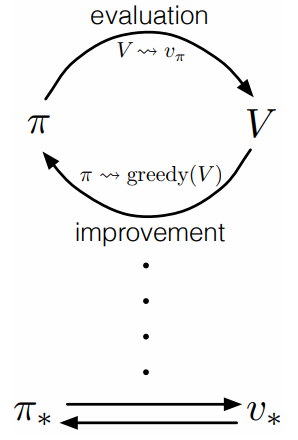
\includegraphics[width=0.3\textwidth]{figures/01/gpi.png}
    \caption{The method of policy iteration, by iteratively evaluation a policy's value function, and subsequently determining the greedy policy for that value function, the policy and value function eventually converges to a fixed iteration point when they are optimal for the given \ac{mdp}.}
    \label{fig:pi}
\end{figure}

This algorithm is proven to converge toward the optimal value function and policy\cite{intro_rl} but with some caveats, namely, it assumes environment knowledge and the curse of dimensionality which will be described further in this text. Nonetheless, the theoretical guarantee for optimality makes it an important foundation method in reinforcement learning and is detailed further. 


\subsubsection{Policy Evaluation}

For a given policy $\pi$, the value function of this policy $v_{\pi}$ is computed by starting with an initial estimate $v_{\pi, 0}$ and recursively applying the Bellman equation on all $s$ as an update rule as shown in \autoref{eq:policy_eval}. This update will be applied until the value function has converged, where convergence can be defined in several ways, the simplest of which is when the norm of the difference between subsequent value functions is smaller than a small constant $\epsilon$.

\begin{equation}\label{eq:policy_eval}
    v_{\pi, k+1}= \sum\limits_{a}\pi(a|s) \sum\limits_{s', r} p(s', r|s, a)[r + \gamma v_{\pi, k}(s')] \quad \forall s \in \mathcal{S}
\end{equation}

Note that to compute the update formulated in \autoref{eq:policy_eval}, the environment dynamics $p(s',r|s,a)$ needs to be known and defined, which is an assumption made during the policy evaluation step.

By inspection of \autoref{eq:state_bellman}, it can be seen that the update equation \autoref{eq:policy_eval} will only converge when the estimation $v_k$ is equal to the true value function $v_{\pi}$.

\subsubsection{Policy Improvement}

For any given value function $v_{\pi}$, an improved policy $\pi'$ is obtained by making $\pi'$ deterministic and greedy with respect to $v_{\pi}$. This is done by defining $\pi'$ to choose the action that has the highest action value in each state $s$:

{\myfont
\begin{equation}\label{eq:policy_improvement}
    \pi'(a|s) = \begin{cases}
    1,& \text{if } a = \underset{a}{\text{argmax}} \ q_{\pi}(s,a) \\
    0,              & \text{otherwise}
\end{cases}
\end{equation}
}

The policy improvement step is guaranteed to find a policy that is at least as good as the previous policy, and in the case of a finite \ac{mdp}, the policy improvement step is guaranteed to find the optimal policy \cite{dp}. After finding a greedy policy on the given value function, the previous value function will no longer be accurate for the new policy \textit{if it is suboptimal for the given \ac{mdp}}. This means that when a policy evaluation step is subsequently performed, a sub-optimal policy will cause the evaluation step to yield a different value function, but an optimal policy will yield the same value function. In other words, this algorithm only converges when the optimal policy and its corresponding value function are determined\cite{intro_rl}.

\subsection{Generalized Policy Iteration}\label{subsec:gpi}

In the policy iteration method just described, the policy evaluation and improvement steps are carried out with the specific update rules in \autoref{eq:policy_eval} and \autoref{eq:policy_improvement}. However, the idea behind policy iteration: evaluating and improving upon some estimated policy or value function, is very useful and can be used to describe on a high level the idea behind many reinforcement learning algorithms as stated by Sutton and Barto \cite{intro_rl}, who they use the term \textit{generalized policy iteration} to capture this idea.

For example, instead of iterating the policy evaluation step until the value function converges, it is possible to only take one or a few iterations and proceed with policy improvement thereafter. This is the idea behind Value Iteration algorithms, which is applied to optimal control problems without using Bellman equations\cite{vi_for_optimal_control, vi_for_optimal_control_2}.

Another example comes from outside of the dynamic programming field, the class of actor-critic can be described using the idea of generalized policy iteration, wherein an estimate of the critic function (the value function) is improved based on sampled transitions from the \ac{mdp}, and the policy function (the actor) is improved using information from the critic.

\subsection{Approximate Dynamic Programming}\label{subsec:adp}
Finite \ac{mdp} are characterized by their discrete and small number of states and actions that are possible, this makes it possible to use dynamic programming to solve for the optimal value function and policy of such a process. However, many systems that are interesting to model and find solutions for have many states and actions possible, and real-life processes frequently have continuous variables instead of discrete ones. Such circumstances can cause a combinatorial explosion in the number of state-action pairs that exist, which means having a specific value and a specific action probability distribution defined for each state becomes impractical. This is the so-called \textit{curse of dimensionality}, alluded to in \autoref{subsec:pi}. Moreover, evaluation of the Bellman equations also requires a known transition probability distribution of the environment. Not only does this also suffer from the curse of dimensionality in the case of large and/or continuous state spaces, but knowledge of such distribution might not be available for some systems, or at the very least inconvenient or difficult to identify. 

One solution to circumvent these issues is to use function approximators for the value function, policy function, and environment model, which leads to the class of dynamic programming based reinforcement learning algorithms called \ac{adp}. In this class, it is common to refer to value functions as \textit{cost-to-go} or \textit{cost} functions instead. Two basic methods exist in this class, the first is the \ac{pi} algorithm whose high-level algorithm is outlined in \autoref{alg:pi}.


\begin{algorithm}[H]
	\caption{Policy iteration, adapted from \cite{pi_and_vi_algorithm}} \label{alg:pi}
	\begin{algorithmic}[1]
        \State \textbf{Initialize}. Define a policy $\pi_0(\mathbf{x}_k)$ which is admissible, i.e. stabilizing, and an arbitrary initial value function $V_0(\mathbf{x})$.
        \State \textbf{Policy Evaluation}. Determine the value function of the current policy using the Hamilton-Jacobi-Bellman Equation:
        \begin{equation}\label{eq:adp_poli_eval}
            V_{i+1}(\mathbf{x}_t) = r(\mathbf{x}_t, \pi_i(\mathbf{x}_t)) + \gamma V_{i+1}(\mathbf{x}_{t+1})
        \end{equation}
        \State \textbf{Policy Improvement}. Determine an improved policy. 
        {\myfont
        \begin{equation}\label{eq:adp_poli_improv}
            \pi_{i+1}(\mathbf{x}_t) = \underset{\pi(\mathbf{x}_t)}{\text{argmin}}[r(\mathbf{x}_t, \pi_i(\mathbf{x}_t)) + \gamma V_i(\mathbf{x}_{t+1})]
        \end{equation}}
        \State If $V_i(\mathbf{x}) \equiv V_{i-1}(\mathbf{x})$ then terminate, else $i = i+1$ and return to step $2$
	\end{algorithmic} 
\end{algorithm}

\autoref{alg:pi} fits into the mold of generalized policy iteration, which incorporates certain aspects of optimal control theory and has some note-worthy aspects. Firstly, the policy evaluation step \autoref{eq:policy_eval} of this algorithm is not formulated in the \ac{mdp} framework like in \autoref{eq:policy_eval}, and instead is the \ac{hjb} equation which is generally difficult to evaluate especially online\cite{frank_lewis_hjb} but can be solved approximately by methods such as least squares approximation using environment observations\cite{ls_approximation}, or by iteratively evaluating the equation until convergence\cite{pi_and_vi_algorithm}. Secondly, instead of the policy being a probability distribution, this algorithm generally uses deterministic policies. Thirdly, if the system dynamics can be formulated as \autoref{eq:normal_system_dynamics} with $n$ and $m$ being the number of state and control variables respectively, and the reward of the system is formulated in a quadratic manner as shown in \autoref{eq:lqr_cost}, then it is known that the policy improvement step takes the form of \autoref{eq:optimal_policy_improvement}\cite{bertsekas2012dynamic}. 

{\myfont
\begin{align*}
    \mathbf{x}_{t+1} & = f(\mathbf{x}_t) + g(\mathbf{x}_t)\mathbf{u}_t \stepcounter{equation}\tag{\theequation}\label{eq:normal_system_dynamics}\\
    r(\mathbf{x}_t, \mathbf{u}_t) &= \mathbf{x}_t^{\top}\mathbf{Q}\mathbf{x}_t + \mathbf{u}_t^{\top}\mathbf{R}\mathbf{u}_t \stepcounter{equation}\tag{\theequation}\label{eq:lqr_cost}\\
    \text{Where} \quad \{\mathbf{x}, f(\mathbf{x})\} \in \mathcal{R}^n, \; g(\mathbf{x}) \in& \mathcal{R}^{n \times m}, \; \mathbf{u} \in \mathcal{R}^m, \; \mathbf{Q} \in \mathcal{R}^{n \times n}, \; \mathbf{R} \in \mathcal{R}^{m \times m}
\end{align*}
}
\begin{equation}\label{eq:optimal_policy_improvement}
    \pi_{i+1}(\mathbf{x}_t) = -\frac{\gamma}{2}\mathbf{R}^{-1}g^{\top}(\mathbf{x}_t)\frac{\partial V_i(\mathbf{x}_{t+1})}{\partial \mathbf{x}_{t+1}}
\end{equation}

The second basic algorithm of the \ac{adp} class is \ac{vi}, whose high-level algorithm is shown in \autoref{alg:vi}.


\begin{algorithm}[H]
	\caption{Value iteration, adapted from \cite{pi_and_vi_algorithm}} \label{alg:vi}
	\begin{algorithmic}[1]
        \State \textbf{Initialize}. Define an arbitrary policy $\pi_0(\mathbf{x}_k)$, and an arbitrary initial value function $V_0(\mathbf{x})$.
        \State \textbf{Policy Evaluation}. Determine the value function of the current policy using the Hamilton-Jacobi-Bellman Equation:
        \begin{equation}\label{eq:adp_poli_eval_vi}
            V_{i+1}(\mathbf{x}_t) = r(\mathbf{x}_t, \pi_i(\mathbf{x}_t)) + \gamma V_i(\mathbf{x}_{t+1})
        \end{equation}
        \State \textbf{Policy Improvement}. Determine an improved policy. 
        {\myfont
        \begin{equation}
            \pi_{i+1}(\mathbf{x}_t) = \underset{\pi(\mathbf{x}_t)}{\text{argmin}}[r(\mathbf{x}_t, \pi_i(\mathbf{x}_t)) + \gamma V_i(\mathbf{x}_{t+1})]
        \end{equation}}
        \State If $V_i(\mathbf{x}) \equiv V_{i-1}(\mathbf{x})$ then terminate, else $i = i+1$ and return to step $2$
	\end{algorithmic} 
\end{algorithm}

Here the same method of policy evaluation and reduction of policy improvement in the \ac{lqr} case holds. The difference between \ac{pi} in \autoref{alg:pi} and \ac{vi} in \autoref{alg:vi} is that the policy evaluation step in \autoref{alg:vi} involves only one evaluation of \autoref{eq:adp_poli_eval_vi}, this is distinguished by the LHS value function having the subscript $i+1$ and the RHS having $i$. Furthermore, \ac{vi} do not require the initial policy to be admissible, which means that to use \ac{vi} algorithms it is not necessary to perform any a priori step on the control policy.

Various forms of these algorithms have been developed further and shown a convergence rate that could allow them to be applied to online control of systems. For instance, Wei et al. \cite{wei_adp} present an optimal control algorithm based on the framework of \ac{adp} using neural networks as function approximations. They demonstrate via simulation of an inverted pendulum control problem that even though their solution of the \ac{hjb} equation is only approximately optimal, by virtue of iteratively performing the police evaluation and improvement steps, their \ac{adp} method can converge to the optimal control law within 5 $s$ or 10 iteration steps. A similar method based on action-value or Q function is proposed by Lin et al. \cite{lin_adp_unknown_system} and demonstrates similar convergence speeds. 

By linearizing a nonlinear system's dynamics, it is possible to perform the policy evaluation and improvement steps in a much more efficient manner. This approach is adopted by zhou et al. \cite{zhou_iadp_1,zhou_iadp_2} who used \ac{rls} regression to identify a linear model at each time step, thus obtaining a time-varying linear model, which reduced the control problem to an \ac{lqr} like problem. Note that this approach relies on a sufficiently high sensor sampling rate, in the order of $10^2\ Hz$, which is needed for the assumption of linear dynamics to hold, as any smooth nonlinear function can be approximated locally by linear functions.

\subsubsection{Multi-step and Eligibility Trace Extensions of ADP Methods}

One trade-off that \ac{adp} methods have to face is between adopting a more policy iteration or a more value iteration approach. In the former approach, algorithms developed generally see faster convergence in their estimates, naturally a desirable characteristic. However, such algorithms require the initial policies to be admissible, otherwise, the control policy would drive the system towards instability, causing the \ac{hjb} equation can grow unbounded. This issue is not faced by the latter approach, as \ac{vi} algorithms do not seek to fully converge towards the optimal solution of the \ac{hjb} equation, instead \ac{vi} only require the value function estimation to be iterated by one step, instead of a large or infinite number of steps.

This binary situation can be reconciled by considering the idea of \textit{multi-step} iterations or updates, which is to take multiple transitions or timesteps worth of information while updating estimates in a reinforcement learning algorithm \cite{intro_rl}.

With the incorporation of a multi-step augmentation to the policy evaluation update rule, this dichotomy is turned into a spectrum of algorithms, where an \ac{adp} method can select how many steps should a policy evaluation iteration take. At the extreme of taking infinite steps, a multi-step \ac{adp} method is simply the \ac{pi} algorithm, on the other extreme, a single-step \ac{adp} method is the \ac{vi} algorithm \cite{mshdp_og}.

A high-level view of the multi-step \ac{adp} algorithm is shown in \autoref{alg:ms_adp}, with $n$ being the number of steps. To make the choice of $n$ automatic, Wang et al. \cite{mshdp_new} derived a criterion for switching $n$ from a low number during the initial iterations of the algorithm, where the initial arbitrary policy is not guaranteed to be admissible, to a high number during the latter iterations when the policy is verified to be admissible under the proposed criterion. 

\begin{algorithm}[H]
	\caption{Multi-step value iteration, known as multi-step heuristic dynamic programming in and adapted from \cite{mshdp_og}.} \label{alg:ms_adp}
	\begin{algorithmic}[1]
        \State \textbf{Initialize}. Define an arbitrary policy $\pi_0(\mathbf{x}_k)$, and an arbitrary initial value function $V_0(\mathbf{x})$.
        \State \textbf{Policy Evaluation}. Determine the value function of the current policy using the multi-step approximation of the Hamilton-Jacobi-Bellman Equation:
        \begin{equation}\label{eq:adp_poli_eval_msvi}
            V_{i+1}(\mathbf{x}_t) =  \gamma^{n} V_i(\mathbf{x}_{t+1}) + \sum\limits_{l=t}^{t+n-1}\gamma^{l-t}r(\mathbf{x}_l, \pi_i(\mathbf{x}_l))
        \end{equation}
        \State \textbf{Policy Improvement}. Determine an improved policy. 
        {\myfont
        \begin{equation}
            \pi_{i+1}(\mathbf{x}_t) = \underset{\pi(\mathbf{x}_t)}{\text{argmin}}[r(\mathbf{x}_t, \pi_i(\mathbf{x}_t)) + \gamma V_i(\mathbf{x}_{t+1})]
        \end{equation}}
        \State If $V_i(\mathbf{x}) \equiv V_{i-1}(\mathbf{x})$ then terminate, else $i = i+1$ and return to step $2$
	\end{algorithmic} 
\end{algorithm}


In a similar vein of leveraging the loose policy condition which \ac{hdp} has, and finding ways of increasing the convergence rate of \ac{hdp}, eligibility traces can also be employed \cite{elig_hdp,elig_gdhp}. Eligibility traces are an alternative method of incorporating additional samples from past timesteps for updating estimates, the objective here is again to improve convergence rates of algorithms, however, the algorithm behind this method is different than multi-step ideas.

Instead of explicitly retrieving samples from certain time steps, eligibility traces simply store the past updates made to the critic or actor, and persistently but at a decaying rate add such updates to the critic or actor for subsequent timesteps. This method is illustrated in \autoref{eq:eligbility_trace}, where $\boldsymbol{\theta}(t)$ is the set or vector of parameters for a certain function approximator at time $t$, this approximator could be the critic or the actor, $\mathcal{E}(t)$ is the eligibility trace at time $t$, and $\Delta \boldsymbol{\theta}(t)$ is the update made to the function approximator at time $t$.

\begin{align*}
    \boldsymbol{\theta}(T+1) &= \boldsymbol{\theta}(t) + \mathcal{E}(t) \stepcounter{equation}\tag{\theequation}\label{eq:eligbility_trace}\\
    \mathcal{E}(t+1) &= \mathcal{E}(t) + \nabla \boldsymbol{\theta}(t) ,\quad \mathcal{E}(0) = 0\\
\end{align*}

\subsection{Adaptive Critic Designs}\label{subsec:acd}

Alongside adaptive dynamic programming, there is a class of algorithms called \ac{acd}. In this class of algorithms, the estimate of value functions is referred to as the \textit{critic}, the critic is thus ``responsible" for policy evaluation; while the estimate of the policy functions is referred to as the \textit{actor}, which is thus ``responsible" for policy improvement. It should be noted that in literature, the terms \ac{adp} and \ac{acd} can be found to be used interchangeably \cite{adp_for_control, acd, old_acd}, notably with the progenitor of \ac{acd} Werbos also using these terms and reinforcement learning interchangeably \cite{vi_for_optimal_control}. Algorithmically, practical implementations of some \ac{adp} and \ac{acd} algorithms are very much alike, as will be stated later during the description of \ac{hdp}. However, in this literature study, the distinction between \ac{adp} being dynamic programming algorithms which are more optimal control-oriented, and \ac{acd} being dynamic programming algorithms which are more reinforcement learning-oriented is made.

Adaptive critic designs can be considered to be reinforcement learning algorithms developed from generalized dynamic programming algorithms \cite{old_acd} whose algorithms are structured similarly to the \ac{pi} \autoref{alg:pi} or the \ac{vi} \autoref{alg:vi}. Just like \ac{adp}, \ac{acd} algorithms are sample efficient enough for entirely online trained controllers to be implemented, which can converge towards a stable controller within a short period of time \cite{tshdp, mshdp_og, adp_for_control}. 

Several main algorithms form the basis of this class: the first and simplest algorithm is \ac{hdp}, the second and slightly more complicated algorithm is \ac{dhp}, and the third but most complicated algorithm is \ac{gdhp}. The increase in complexity comes from what the critics of each algorithm estimate, where \ac{hdp} only estimates the value function, \ac{dhp} estimates the gradient of the value function, and \ac{gdhp} estimates both the value and gradient of the value functions. Two extensions of all three of these basic algorithms exist, the first kind of extension makes the critic function \ac{ad}, which changes the critic from being an estimate of the state-value function to an estimate of the action-value function \cite{og_action_dependent}. The second kind of extension changes how the model estimate is obtained, where an \ac{rls} regressor is used to identify linear systems for the immediate time steps, as opposed to using online supervised learning with neural networks or with offline identified models. This class of algorithms is summarized in \autoref{fig:acd}.

\begin{figure}[H]
    \centering
    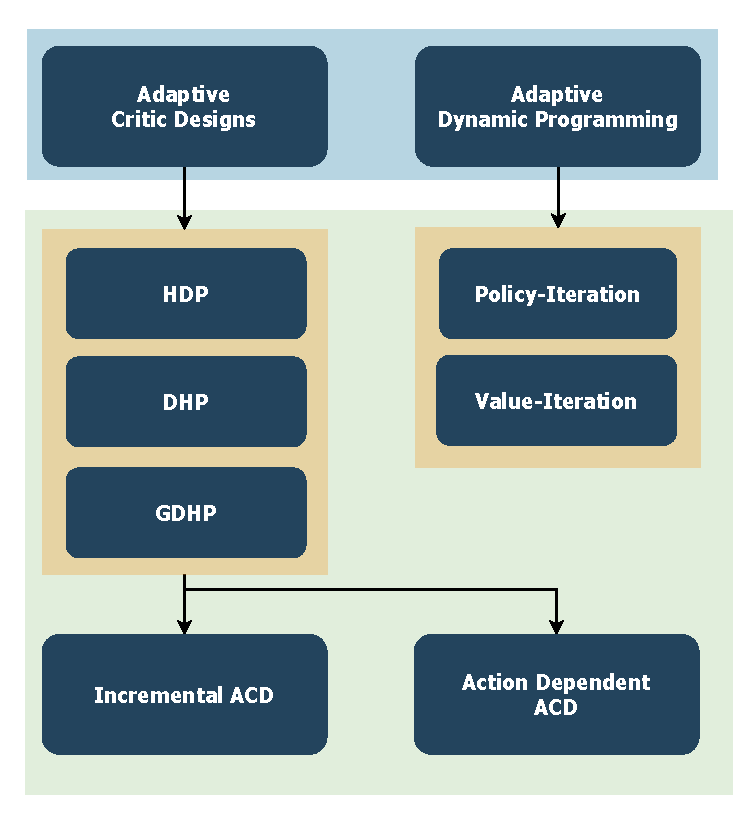
\includegraphics[width=0.7\textwidth]{figures/01/acd.pdf}
    \caption{Overview of Adaptive Critic Design algorithms}
    \label{fig:acd}
\end{figure}


In the \ac{acd} context, the value function is often called the cost-to-go function, but its definition remains the same as the return expected from a given state; the rewards also have a different name, and are sometimes called the one-step costs. 

\begin{align*}
    V(\mathbf{x}_t) &= r_t + \gamma V(\mathbf{x}_{t+1}) \stepcounter{equation}\tag{\theequation}\label{eq:acd_value_function}\\
    r_t &= \frac{1}{2}(\mathbf{x}_t - \mathbf{x}_{t, ref})^{\top}(\mathbf{x}_t - \mathbf{x}_{t, ref})\stepcounter{equation}\tag{\theequation}\label{eq:acd_reward}
\end{align*}
\subsubsection{Heuristic Dynamic Programming}

\ac{hdp} is characterized by using the critic to estimate the value function $V(\mathbf{x}_t)$ itself:

This critic is evaluated by the critic \ac{td} error $\mathbf{e}_c(t)$ defined in \autoref{eq:hdp_critic_td}, and is trained to minimize the critic error function \autoref{eq:hdp_critic_error_function}. To perform training, the function approximator of the critic is updated using a gradient descent method to minimize the error function, meaning the parameters $\boldsymbol{\theta}(t)$ are updated according to \autoref{eq:hdp_critic_update}.

\begin{align*}
    \mathbf{e}_{1,c}(t) &= V(\mathbf{x}_t) - r_t - \gamma V(\mathbf{x}_{t+1}) \stepcounter{equation}\tag{\theequation}\label{eq:hdp_critic_td}\\
    \mathbf{E}_c(t) &= \frac{1}{2}\mathbf{e}_{1,c}(t)^{\top}\mathbf{e}_{1,c}(t) \stepcounter{equation}\tag{\theequation}\label{eq:hdp_critic_error_function}\\
    \boldsymbol{\theta}_c(t+1) &= \boldsymbol{\theta}_c(t) - \nabla \boldsymbol{\theta}_c(t) \stepcounter{equation}\tag{\theequation}\label{eq:hdp_critic_update}\\
    \text{Where} \quad \nabla \boldsymbol{\theta}_c(t) &= \eta_c \frac{\partial \mathbf{E}_c(T)}{\partial \boldsymbol{\theta}_c(t)} = \eta_c \frac{\partial \mathbf{E}_c(T)}{\partial \mathbf{e}_{1,c}(t)}\frac{\partial \mathbf{e}_{1,c}(t)}{\partial V(\mathbf{x}_t)}\frac{\partial V(\mathbf{x}_t)}{\partial \boldsymbol{\theta}_c(t)}
\end{align*}

Correspondingly, there is also the actor loss, the actor error function, and the actor update rule that are expressed in the following equations:

\begin{align*}
    \mathbf{e}_a(t) &= V(\mathbf{x}_t) \stepcounter{equation}\tag{\theequation}\label{eq:hdp_actor_td}\\
    \mathbf{E}_a(t) &= \frac{1}{2}\mathbf{e}_a(t)^{\top}\mathbf{e}_a(t)\stepcounter{equation}\tag{\theequation}\label{eq:hdp_actor_error_function}\\
    \boldsymbol{\theta}_a(t+1) &= \boldsymbol{\theta}_a(t) - \nabla \boldsymbol{\theta}_a(t) \stepcounter{equation}\tag{\theequation}\label{eq:hdp_actor_update}\\
    \text{Where} \quad \nabla \boldsymbol{\theta}_a(t)= \frac{\partial \mathbf{E}_a(t+1)}{\partial \boldsymbol{\theta}_a(t)}  &= \frac{\partial \mathbf{E}_a(t+1)}{\partial \mathbf{e}_a(t+1)}\frac{\partial \mathbf{e}_a(t+1)}{\partial V(\mathbf{x}_{t+1})} \frac{\partial V(\mathbf{x}_{t+1})}{\partial \mathbf{x}_{t+1}} \frac{\partial \mathbf{x}_{t+1}}{\partial \mathbf{u}_t} \frac{\partial \mathbf{u}_t}{\partial \boldsymbol{\theta}_a(t)} \stepcounter{equation}\tag{\theequation}\label{eq:hdp_actor_weight_chainrule}\\
\end{align*}

Observing the formulation of \ac{hdp} thus far presented, an interesting note can be made of the close resemblance in the practical implementation of \ac{hdp} and \ac{pi} or \ac{vi} algorithms or even the interchangeable use of \ac{adp} with \ac{hdp} \cite{costate_adp, policy_iteration_adp, mshdp_og}.

Observing the update equations, it can be seen that the actor update contains the partial derivative $\frac{\partial \mathbf{x}_{t+1}}{\partial \mathbf{u}_t}$, this is a derivative that needs to be obtained using a system model which would define the relation between the state $\mathbf{x}_{t+1}$ and the action $\mathbf{u}_t$. As a result, this makes the \ac{hdp} algorithm model-dependent. However, this dependency can be removed if \ac{hdp} is made \ac{ad}, in which case the value function would be a function of both state and action $V(\mathbf{x}_t, \mathbf{u}_t)$, this allows the chain rule expansion in \autoref{eq:hdp_actor_weight_chainrule} to reduce the term $\frac{\partial V(\mathbf{x}_{t+1})}{\partial \mathbf{x}_{t+1}} \frac{\partial \mathbf{x}_{t+1}}{\partial \mathbf{u}_t}$ to only $\frac{\partial V(\mathbf{x}_{t+1})}{\partial \mathbf{u}_t}$ since $V$ would be an explicit function of $\mathbf{u}_t$, thus eliminating the system dynamics $\frac{\partial \mathbf{x}_{t+1}}{\partial \mathbf{u}_t}$.

An alternative way of alleviating model dependency is to use the incremental method of Zhou et al., who developed the \ac{ihdp} algorithm and successfully applied it to several tasks, including a flight control task \cite{ihdp}, and a launch vehicle control task \cite{ihdp_lv}. In this case, the partial $\frac{\partial \mathbf{x}_{t+1}}{\partial \mathbf{u}_t}$ can be replaced by a control effectiveness matrix from an online identified linear system. Note that this does not make the algorithm entirely model free, since the formulation of the update rules still involves using system dynamics, i.e requires environment modeling.

This algorithm performs relatively poorly compared to \ac{dhp} and \ac{gdhp} in terms of control performance and disturbance rejection \cite{dhp_vs_hdp, old_acd}, but nonetheless have been deployed successfully \cite{adhdp_use_1, adhdp_use_2, hdp_use}.

\subsubsection{Dual Heuristic Programming}

\ac{dhp} is characterized by the critic estimating the gradient of the value function $\lambda(\mathbf{x}_t)$, instead of the value function directly. This gradient can also be referred to as the \textit{costate} \cite{pi_and_vi_algorithm}:

\begin{equation}\label{eq:costate}
    \lambda(\mathbf{x}_t) = \frac{\partial V(\mathbf{x}_t)}{\partial \mathbf{x}_t}
\end{equation}

Here, the actor formulation is identical to the \ac{hdp} algorithm, and only the critic formulations are changed. The critic \ac{td} error is now defined using gradients of the value function, as shown in \autoref{eq:dhp_critic_td}, with the critic error function and function parameter update remaining unchanged.


\begin{align*}
    \mathbf{e}_{2,c}(t) &= \lambda(\mathbf{x}_t) - \frac{\partial r_t}{\partial \mathbf{x}_t} - \gamma \lambda(\mathbf{x}_{t+1}) \frac{\partial \mathbf{x}_{t+1}}{\partial \mathbf{x}_t}\stepcounter{equation}\tag{\theequation}\label{eq:dhp_critic_td}\\
    \mathbf{E}_c(t) &= \frac{1}{2}\mathbf{e}_{2,c}(t)^{\top}\mathbf{e}_{2,c}(t)  \stepcounter{equation}\tag{\theequation}\label{eq:dhp_critic_error_function}\\
    \boldsymbol{\theta}_c(t+1) &= \boldsymbol{\theta}_c(t) - \nabla \boldsymbol{\theta}_c(t) \stepcounter{equation}\tag{\theequation}\label{eq:dhp_critic_update}\\
    \text{Where} \quad \nabla \boldsymbol{\theta}_c(t) &= \eta_c \frac{\partial \mathbf{E}_c(T)}{\partial \boldsymbol{\theta}_c(t)} = \eta_c \frac{\partial \mathbf{E}_c(T)}{\partial \mathbf{e}_{2,c}(t)}\frac{\partial \mathbf{e}_{2,c}(t)}{\partial \lambda(\mathbf{x}_t)}\frac{\partial \lambda(\mathbf{x}_t)}{\partial w_c(t)}
\end{align*}

With this variation, the model-dependency of the algorithm has increased, as the critic \ac{td} error also uses the system dynamics in the form of $\frac{\partial \mathbf{x}_{t+1}}{\partial \mathbf{x}_t}$ in its formulation. Here, introducing an \ac{ad} variant will not remove the model dependence from the algorithm entirely, only from the actor component.

Because the critic function in \ac{dhp} directly outputs value function gradients, which are needed in actor updates, there are no additional numerical errors that get injected into the actor function parameter update, which cannot be said for the \ac{hdp} algorithm. 

This algorithm is extended to an incremental model identification version, resulting in \ac{idhp}. Application of \ac{idhp} to the task of flight control demonstrated improved reference tracking performance and fault tolerance than a pure \ac{dhp} algorithm \cite{idhp, heyer_idhp},  wherein the \ac{idhp} controller was able to recover control of the simulated aircraft even after the flight dynamics were reversed mid-flight. 

\subsubsection{Globalized Dual Heuristic Programming}
\ac{gdhp} is characterized by the critic estimating the value and gradient of the value function simultaneously, thus the critic can be treated as returning a vector of value-function variables $\begin{bmatrix}
        V(\mathbf{x}_t) &
        \lambda(\mathbf{x}_t)
    \end{bmatrix} ^{\top}$.

This results in the \ac{gdhp} critic error function being composed of two terms, a \ac{hdp} and a \ac{dhp} td error

\begin{align*}
    \mathbf{E}_c(t) &= \frac{1}{2}\mathbf{e}_{1,c}(t)^{\top}\mathbf{e}_{1,c}(t)   + \frac{1}{2}\mathbf{e}_{2,c}(t)^{\top}\mathbf{e}_{2,c}(t) \stepcounter{equation}\tag{\theequation}\label{eq:gdhp_critic_error_function}\\
    \boldsymbol{\theta}_c(t+1) &= \boldsymbol{\theta}_c(t) - \nabla \boldsymbol{\theta}_c(t) \stepcounter{equation}\tag{\theequation}\label{eq:gdhp_critic_update}\\
    \text{Where} \quad \nabla \boldsymbol{\theta}_c(t) = \eta_c \frac{\partial \mathbf{E}_c(T)}{\partial \boldsymbol{\theta}_c(t)}  &= \eta_c \bigg(\frac{\partial \mathbf{E}_c(T)}{\partial \mathbf{e}_{1,c}(t)} \frac{\partial \mathbf{e}_{1,c}(t)}{\partial V(\mathbf{x}_t)} \frac{\partial V(\mathbf{x}_t)}{\partial \boldsymbol{\theta}_c(t)} + \frac{\partial \mathbf{E}_c(T)}{\partial \mathbf{e}_{2,c}(t)} \frac{\partial \mathbf{e}_{2,c}(t)}{\partial \lambda(\mathbf{x}_t)} \frac{\partial \lambda(\mathbf{x}_t)}{\partial \boldsymbol{\theta}_c(t)}\bigg) \stepcounter{equation}\tag{\theequation}\label{eq:gdhp_critic_weight_chainrule}\\
\end{align*}

\ac{gdhp} are theoretically superior to both \ac{hdp} and \ac{dhp} since its critic estimates both the outputs of their respective critics, but the two common implementations of \ac{gdhp} both have practical issues. In the first common implementation, the \ac{gdhp} critic only outputs the value function \cite{igdhp_erik, gdhp_impl1} and the partial derivative $\frac{\partial \lambda(x_t)}{\partial w_c(t)}$ from \autoref{eq:gdhp_critic_weight_chainrule} is then computed by replacing it with the partial derivative $\frac{\partial^2 V(x_t)}{\partial x_t \partial w_c(t)}$, which is computationally expensive and practically complicated to implement. The second common implementation of \ac{gdhp} involves using one function approximator for the critic, which outputs both the value function and its gradient \cite{fault_tolerant_gdhp, gdhp_impl2_a, gdhp_impl2_b}, just as stated at the beginning of this subsection. However, in such implementations, the gradient of the value function is not guaranteed to be an accurate estimate of the gradient.

Reconciling the two issues of computational complexity and analytical accuracy, Zhou \cite{zhou_igdhp} proposed the idea of building the critic as two function approximations but with a novelty of formulating the $\lambda(x_t)$ approximator based explicitly on the $V(x_t)$ approximator, which was applied to a longitudinal flight control task, and shows promising capacity in being able to reap the simultaneous benefit of efficiency and accuracy.


\section{Deep Reinforcement Learning}

Besides Adaptive Dynamic Programming, the other major field of reinforcement learning research is \ac{drl}. Both of these fields revolve around using function approximators \cite{function_approximators} to address the curse of dimensionality which hinders the deployment of reinforcement learning algorithms to real-life problems, which often contain many continuous variables. A big distinction between these fields is how \ac{drl} stems largely from deep learning methods, where deep neural networks are used as the function approximator or incorporated in any other way into algorithms. The types of algorithms belonging to this class are summarized in \autoref{fig:drl}. As can be seen, \ac{drl} is separated into various classes of algorithms and this section will describe each one of these classes, in addition to presenting notable algorithms from each class.


\begin{figure}[H]
    \centering
    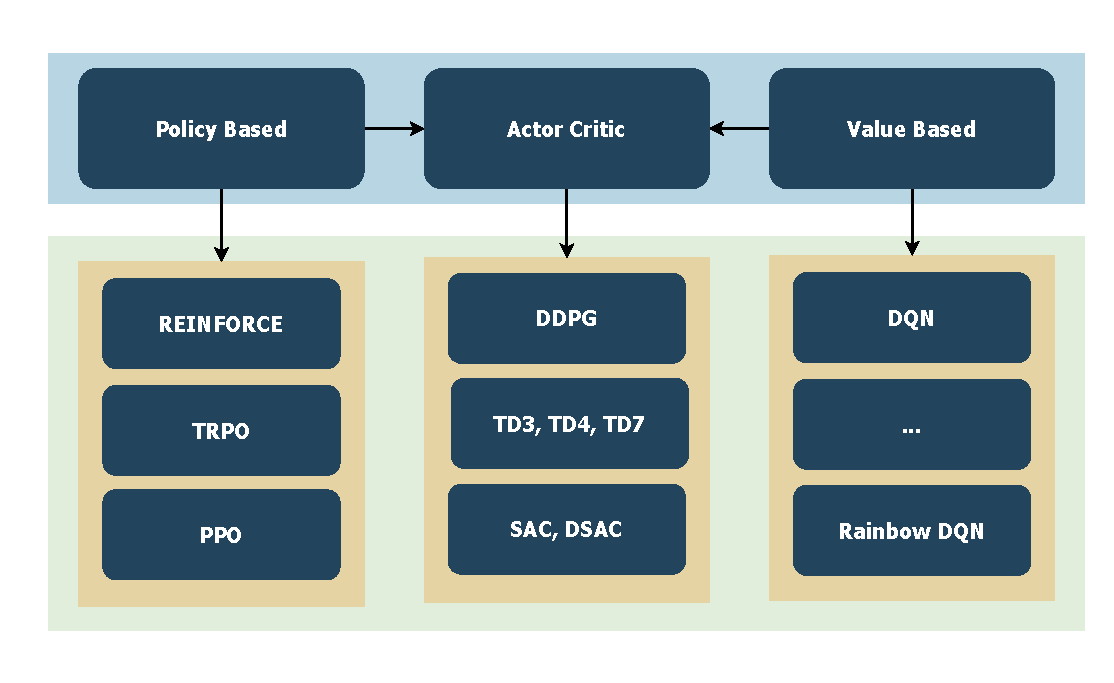
\includegraphics[width=0.7\textwidth]{figures/01/drl.pdf}
    \caption{Overview of deep reinforcement learning algorithms}
    \label{fig:drl}
\end{figure}

This section is laid out as follows, first a description of deep learning is given in \autoref{subsec:deep_learning}, then value-based methods are discussed in \autoref{subsec:value_based_drl}, followed by policy-based methods in \autoref{subsec:policy_based_drl}, and lastly a discussion on the combination of policy and value-based methods called actor-critic methods in \autoref{subsec:ac_drl}.

\subsection{Deep Learning}\label{subsec:deep_learning}

Deep learning refers to the subfield of machine learning which studies deep neural networks and their applications. This field has its origins in the ideas of artificial neural networks and is a scientific effort that has dramatically changed the idea of what an artificial neural network is and what it might be capable of. Deep neural networks fundamentally are an expansion of artificial neural networks, they use the same basic architecture of a neural network, with layers of interconnected neurons between a surface or input layer and a final output layer. One distinction between deep and artificial neural networks is that deep neural networks use many more layers and nodes than are typical in artificial networks. In addition to deep neural networks, deep learning also encompasses many other types of neural networks, a short list of some network types under deep learning and their descriptions are listed below.

\begin{enumerate}
    \item \textbf{\ac{dnn}}. Neural networks with a large number of neurons and hidden layers. From the \textit{Universal Approximation Theorem}, it is known that neural networks are capable function approximators, and were pioneered to do as such \cite{dnn_pioneer_for_function_approximation}. The large network structure of \acp{dnn} allows them to be trained more efficiently to approximate a given function \cite{Liang2016WhyDN}, in addition to allowing them to approximate more nonlinearities.
    \item \textbf{\ac{cnn}}. Neural networks that contain convolutional layers that processes the input into a map of features detected. Pioneered in handwritten number detection \cite{cnn_og}, incorporating convolution into neural networks allows for detecting and utilizing patterns that may exist in the input data.
    \item \textbf{\ac{rnn}}. Neural networks that feed their output back as input, or have some form of memory component. Their architecture makes them more applicable to temporal data than other network architectures and is popular for generative predictive sequences in for example text writing \cite{rnn_4_writing} and language modeling \cite{rnn_4_language}.
\end{enumerate}

Deep learning had several groundbreaking results before practitioners of reinforcement learning managed to apply some of the advances into their own algorithms, such as in the area of computer vision \cite{dnn_b4_drl_1_image_recognition, dnn_b4_drl_2_image_recognition}, speech recognition \cite{dnn_b4_drl_1_speech_recognition, dnn_b4_drl_2_speech_recognition}, and in handwriting generation \cite{rnn_4_writing}. These results demonstrated that deep neural networks had the power to use the same raw data which humans perceive, and interpret useful information out of them, or even generate new information. So it seemed only natural to see if it was possible to combine the learning emulation of reinforcement learning, with the world processing emulation of deep learning, to produce machines that could perceive \textit{and} learn from the world just as humans do. This ethos is notably different from that of \ac{adp} or \ac{acd}, as here the emphasis is on recreating the way which humans and animals interact with an environment, rather than on extending mathematical theory.

\subsubsection{DNNs for Function Approximation}

A generic neural network layer can be denoted as a vector function $f(\mathbf{x})$ in the following manner:

\begin{equation}\label{eq:generic_layer}
    f(\mathbf{x}) = g(\boldsymbol{\theta}\mathbf{x} + \mathbf{b})
\end{equation}

With $\boldsymbol{\theta}$ a square weight matrix, $\mathbf{b}$ a vector of biases, and $g(\cdot)$ an arbitrary activation function, preferably differentiable. To build a full network such as a \ac{dnn}, one simply has to use the output of one layer as the input of a subsequent layer:

\begin{equation}\label{eq:generic_dnn}
    \mathbf{y} = h(\mathbf{x}) = f_1(f_2(\dots(f_k(\mathbf{x}))))
\end{equation}

Just as the case in \ac{adp} and \ac{acd}, when \ac{dnn} is being used as the function approximator, the weights and biases parameterizing the network are the values that need to be updated during training. These updates are done in such a way that improvements in estimate accuracy are observed, which can be done by gradient descent.

The specific gradient descent method used to optimize parameters in neural networks is called \textit{backpropagation}, which is the name given to the broad method of determining the derivative of the entire set of parameters. This method uses, the gradient of the network's \textit{loss function} $J$, which measures the accuracy of the network's prediction, with respect to all the weight and biases of the network, to provide the increment on each parameter that would result in the lowest loss. When $g_k(\cdot)$ is differentiable everywhere, this gradient will always be defined, when that is not the case, numerical errors may propagate through the network update thus differentiability for $g(\cdot)$ is generally desired.

This partial derivative in practice can be calculated very efficiently, as all the information needed is present during one feedforward step of the network.

For the main step of optimizing values of weights and biases, this gradient is used with an optimizer to determine the increment applied to each parameter \cite{gradient_optimizers}. A popular option in \ac{drl} is \ac{sgd}, the stochastic in this optimizer's name refers to the fact that this optimizer uses one training sample to determine a gradient, which is stochastic as the training sample is essentially one realisation of a random process. This single sample gradient is then scaled by a learning rate $\eta$  \ac{sgd} is an easy-to-understand and implement optimizer, but is rudimentary in comparison to other optimizers. \ac{sgd} nonetheless forms the basis for many gradient optimizer algorithms, and the parameter update rule using \ac{sgd} is shown as follows:

\begin{equation}
    \boldsymbol{\theta}_{t+1} = \boldsymbol{\theta}_t - \eta \nabla J(\boldsymbol{\theta}_t)
\end{equation}
One improved optimizer is the Adagrad optimizer, which is based on \ac{sgd} but features a variable $\eta$ which adapts to each parameter, such that the size of a parameter's update is based on the frequency that the parameter is updated; these changes make Adagrad particularly suitable when training data is sparse \cite{gradient_optimizers}.


\subsection{Value Based Deep Reinforcement Learning}\label{subsec:value_based_drl}

Value-based \ac{drl} algorithms focus on the estimation of the optimal value function $Q^*(s,a)$ using \acp{dnn} as function approximators, resulting in an approximate value function $Q(s,a,\theta_c)$ parameterized by some parameters $\theta_c$, and have a relatively simple policy component that picks the action which has the maximum value according to the value estimates, i.e. picks the greedy action. It is sometimes desirable to not always act greedily, and to instead pick the actions estimated to be suboptimal with some small probability $\epsilon$ in order to facilitate exploration, a so-called $\epsilon$ greedy strategy: 

\begin{equation}
    \pi'(a|s) = \begin{cases}
    1-\epsilon,& \text{if } a = \underset{a}{\text{argmax}} \ q_{\pi}(s,a) \\
    \epsilon ,              & \text{otherwise}
    \end{cases}, \quad 0 < \epsilon < 1
\end{equation}


\subsubsection{Deep Q Network}
The first successful \ac{drl} algorithm came from the value-based approach, and it was the \ac{dqn} algorithm \cite{dqn}. It was a model-free algorithm that managed to successfully use pixel-based sensory input to learn control policies for a series of Atari games. The algorithm is based on Q-learning, in the tabular case this would mean using either the temporal difference learning method or the \ac{mc} learning method to iteratively update an estimate for the action-value function of all state-action pairs. Here, the dimension of the state space was immense, because frames of gameplay footage are used as pixel-based sensory information. Thus it is logical to use a \ac{cnn} as a function approximator for the action-value function, called the \textit{Q-network}, instead of discretely recording the action value for every combination. This algorithm had two features that contributed largely to its success, they were: \textit{Expereience Replay} and \textit{Target Network}. 

\begin{itemize}
    \item \textbf{Experience Replay} \cite{dqn}. Deep learning typically assumes samples to be independent, which is untrue for samples in reinforcement learning problems and can result in biases introduced to the Q-network estimates. To reduce the correlation between samples, the agent's experienced transition tuples $(s_t, a_t, r_t, s_{t+1})$ are stored in a queue memory-buffer with a limited size $n$; and training of the Q-network is done by sampling a transition randomly from this queue, and updating the value estimate associated with the state transition of this sample with the recorded reward.
    \item \textbf{Target Network} \cite{dqn}. The target here is the value that a value estimate is moved towards, as described in \autoref{sec:basic_rl_algo}. Learning instability can arise when targets change too rapidly, which can be the case if the targets are taken from the estimated Q-network. Hence, a separate \textit{target} Q-network is stored, from which the update targets are retrieved and whose weights are only periodically synchronized with the estimated Q-network. Thus ensuring the targets do not vary drastically from update to update. 
\end{itemize}

The problems that these two features aim to tackle are universal in reinforcement learning, and while other techniques to address these challenges of sample correlation and learning stability exist, the two features augmented to \ac{dqn} can be useful in other algorithms as well.

\subsubsection{Rainbow DQN and other improvements}

Many independent experiments and improvements were made to the architecture of DQN and other reinforcement learning algorithms, each of which addressed an issue separate from the other, van Hasselt et al. compiled a list of such ingredients for an algorithm and combined them into one single \ac{dqn} value based algorithm called Rainbow \ac{dqn} \cite{rainbow_dqn}. These various modules are compiled in the following list:

\begin{itemize}
    \item \textbf{Double Learning} \cite{ddqn}. Originally proposed in the tabular setting, the idea of double learning is to keep and learn two estimates of the value function at the same time, with either one of the two networks being randomly chosen to be trained for any given experience sample. Doing so reduces the value estimates, which are overly optimistic due to the bias arising from the usage of the {\myfont argmax} operator \cite{double_q_learning}. 
    \item \textbf{Prioritized Experience Replay} \cite{prioritized_exp_replay}. When learning under the experience replay framework, the transitions from the memory-buffer are sampled with uniform probability. This can be suboptimal considering that some transitions do not contain significant information on the environment, and thus do not train the agent as well as it would have been trained if another transition was sampled. By assuming transitions that result in a higher \ac{td} error as being more important for learning, and sampling such transitions with higher probability, it has been shown that an agent's rate of learning improves, i.e. sample efficiency can be raised.
    \item \textbf{Duelling Network Architecture} \cite{dueling_architecture}. A novel neural network architecture, named \textit{dueling architecture}, is adopted to approximate the value function estimates. The dueling architecture is distinguished by the output layer being preceded by two streams of separate hidden layers, the first stream being used to estimate state-value functions, while the second is used to estimate action advantages -a similar variable to the action value-. Preceding these two streams is one common convolutional network, laid out in a similar manner as the convolutional layers in the original \ac{dqn} algorithm. By utilizing this dueling architecture, the complexity of learning for the neural network is reduced, which contributes towards higher sample efficiency and better agent performance.
    \item \textbf{Multi-step Bootstrapping} \cite{intro_rl, a3c}. The basic approach in bootstrap learning algorithms and thus in most value-based methods is to use the reward from a single transition as the learning target. As suggested by Sutton \cite{Sutton_multi_step} and corroborated in \ac{adp} research \cite{mshdp_og}, taking multiple timesteps worth of transitions to form a learning target can produce faster learning rate, as it allows rewards to be propagated throughout the domain of the estimate faster \cite{Sutton_multi_step}. This variation was used on four standard algorithms by Mnih et al. \cite{a3c}, where the idea was brought further to using transitions from several asynchronously trained agents, which defined a class of asynchronous algorithms with agents trained on separate computing units.
    \item \textbf{Distributional Learning} \cite{distributional_rl_1, distributional_rl_2}. Whereas the traditional reinforcement learning paradigm is concerned with \textit{expected} values, there is also a view that studying the distribution of values can be incorporated into learners, which should allow for more risk-aware behaviours, and intuitively allows agents to make use of more information than merely the expectation of a random variable. A commonly used analogy is that distributional learning is to treat the environment observations as colours pictures, while expectational learning is to treat it as black-and-white pictures. To make use of distributional reinforcement learning, an estimate for the distribution of returns and thus of the state or action-values are learned, specifically the first and second moments of the distribution \cite{distributional_rl_1}.
    \item \textbf{Noisy networks} \cite{noisy_networks}. The problem of exploration vs exploitation is important for algorithms to address, noisey networks seek to provide a means of finetuning the degree of exploration built into an algorithm. A noisy network is made by adding random values to the weights and biases to any neural network, which can be done to any given network as well as other forms of function approximators. The advantage that such an augmentation brings to algorithms is by allowing estimates to escape local optima, increasing the likelihood of encountering the global optimum by virtue of traversing the domain more widely.
\end{itemize}


\subsection{Policy Based Deep Reinforcement Learning}\label{subsec:policy_based_drl}
Policy-based methods, also known as policy search methods, primarily optimize the policy of an agent as opposed to the value function, and can select actions without the need to consult value functions, but can reap benefits by simultaneously estimating values as will be discussed in \autoref{subsec:ac_drl}. The policy $\pi(a|s,\boldsymbol{\theta_a})$ in such methods is approximated with a \ac{dnn} parameterized with the parameters $\boldsymbol{\theta_a}$. By training for an optimal policy directly, instead of training a value function on which a policy will be inferred, one layer of complexity is removed from the training task.

The foundation of policy-based methods is based upon the \textit{policy gradient theorem}, which is an analytical expression derived from the Bellman equations of \autoref{eq:state_bellman} which defines the gradient of a policy's performance or optimality with respect to the policy parameters, this gradient is called the \textit{policy gradient}. According to this theorem, the following proportionality for the gradient of a policy's loss holds true:

\begin{equation}
    \nabla J(\boldsymbol{\theta_a}) \propto \sum\limits_s \mu(s) \sum\limits_a q_{\pi}(s,a)\nabla \pi(a|s,\boldsymbol{\theta_a})
\end{equation}

Where $\mu(s)$ is the state distribution which describes the importance of each state, which is related to how often a state is visited, and thus is theoretically a function of the policy parameters since the policy decides what action and thus what states might be visited. The Important result of this theorem is that this expression shows that policy gradient does not require taking the gradient of $\mu(s)$, despite it being technically a function of policy parameters, which makes it much easier to implement gradient descent routines to optimize a policy \cite{intro_rl}.

\subsubsection{REINFORCE}

The simplest form of policy-based method is called REINFORCE, which is an acronym for the form of the algorithm: REward Increment = Nonnegative Factor $\times$ Offset Reinforcement $\times$ Characteristic Eligibility \cite{williams1992simple}. REINFORCE uses the \ac{mc} learning approach to train its policy network, where the parameter updates to the policy are only performed at the end of each episode. The parameter update rule of REINFORCE is expressed as follows \cite{intro_rl}:

{\myfont
\begin{equation}\label{eq:reinforce_update}
    \boldsymbol{\theta}_{t+1} = \boldsymbol{\theta}_t + \eta G_t \nabla \ln(\pi(A_t|S_t, \boldsymbol{\theta}_t))
\end{equation}
}

In this update rule, every parameter update is proportional to the return observed $G_t$ for each state-action pair $S_t A_t$., and it is in the direction of the vector represented by {\myfont$\nabla \ln()$}, which is the direction in parameter space that contains policies which have a higher likelihood of repeating action $A_t$ when in state $S_t$. This update is thus logical since if a state action pair has a high return, it would be beneficial to update the policy to enact such actions more, which is exactly what the update term in \autoref{eq:reinforce_update} does. 

\subsubsection{Trust Region Policy Optimization}

The theoretical convergence properties of REINFORCE are very positive, in the expectation this algorithm is guaranteed to improve the policy \cite{williams1992simple, intro_rl}. In practice, algorithms revolving around the REINFORCE framework have very low sample efficiency and thus are slow to converge, in addition to high variance in learning rate. One way of circumventing these deficiencies is to incorporate baselines that modulate the magnitude of policy parameter updates, thus reducing learning variance. An extension of this idea is the \ac{trpo} algorithm proposed by Schulman et al.

\ac{trpo} effectively reduces the variance of policy updates through constraining update steps when the parameter updates are too aggressive \cite{trpo}, this aggressiveness is determined by measuring the distance between the original policy and the updated policy. Since a policy function is a probability distribution, measuring the distance between policies thus requires using probability distance measures, in the case of \ac{trpo} this distance measure is the \ac{kl} divergence; returning a scalar value representing how different the two probability distributions are \cite{kullback1951information}. 

This algorithm casts the policy-gradient method as an optimization problem, which is formulated as follows:

{\myfont
\begin{align*}
    \underset{\boldsymbol{\theta}_a}{\text{maximize }} \ &\mathbb{E} \bigg[\frac{\pi(a|s,\boldsymbol{\theta}_a)}{\pi(a|s, \boldsymbol{\theta}_{a,old})} Q_{\pi_{old}}(s,a)\bigg] \stepcounter{equation}\tag{\theequation}\label{eq:trpo_opt_problem}\\
    \text{subject to }\  &\mathbb{E} \big[ D_{KL}\big(\pi(\cdot|s, \boldsymbol{\theta}_a) || \pi(\cdot |s, \boldsymbol{\theta}_{a, old})\big)\big] \leq \delta
\end{align*}
}

Being a policy-based method, no function is used to approximate the action-values $Q_{\pi}(s,a)$. Instead, $\pi$ is executed over some number of time steps generating a trajectory, and these values are estimated using samples from the trajectory.

Formulating the policy learning problem as an optimization problem is noticeably divergent from all algorithms thus far presented, indeed this approach of addressing the reinforcement learning problem is a field of research in itself, such as in the \ac{drl} subfield of policy search \cite{deisenroth2013survey} and evolutionary reinforcement learning \cite{erl}. The optimization problem from \autoref{eq:trpo_opt_problem} is then solved using conjugate gradient optimization algorithms. The specific optimization algorithm proposed by Schulman et al to solve the \ac{trpo} problem uses Hessian matrices and thus can be considered to be a second-order algorithm.

Despite the reduced learning variance benefits that this algorithm has over REINFORCE, \ac{trpo} remains complicated to implement, uses the \ac{kl} divergence measure which is computationally expensive due to the optimization algorithm posed, while suffering from slow learning rates \cite{ppo}. Hence, more augmentations are needed.

\subsubsection{Proximal Policy Optimization}

When the policy-gradient algorithms were cast into an optimization problem, as done by Schulman et al. through \ac{trpo}, this opened up new possibilities for making changes to policy-gradient algorithms. For one, instead of posing a constrained optimization problem as done in \autoref{eq:trpo_opt_problem}, an unconstrained optimization problem can be formulated by stating the optimization constraints as penalties in the objective function being maximized, resulting in the optimization problem posed by \autoref{eq:ppo_optimization} with a tunable parameter $\beta$.

{\myfont
\begin{equation}\label{eq:ppo_optimization}
    \underset{\boldsymbol{\theta}_a}{\text{maximize }} \ \mathbb{E} \bigg[\frac{\pi(a|s,\boldsymbol{\theta}_a)}{\pi(a|s, \boldsymbol{\theta}_{a,old})} A_{\pi_{old}}(s,a) - \beta D_{KL} [\pi(\cdot | s, \boldsymbol{\theta}_a) || \pi(\cdot |s, \boldsymbol{\theta}_{a, old})]\bigg] 
\end{equation}
}

In fact, \autoref{eq:ppo_optimization} is the optimization problem suggested by the theory which justifies \ac{trpo} \cite{ppo}. However, the presence of $\beta$ makes this objective function difficult to define, thus surrogate objective functions are formulated to pose essentially the same optimization problem as \autoref{eq:ppo_optimization}. Such a surrogate objective function $J_{CLIP}(\boldsymbol{\theta}_a)$ is defined in \autoref{eq:ppo_surrogate_optimization}, it has a tunable parameter $\epsilon$ and uses the \textit{advantage function} $A_{\pi}(s,a)$, and is the loss function that creates the \ac{ppo} algorithm.

{\myfont
\begin{align*}
        \underset{\boldsymbol{\theta}_a}{\text{maximize }} J_{CLIP}(\boldsymbol{\theta}_a) = &\mathbb{E} \bigg[\text{min}\bigg( r(\boldsymbol{\theta}_a), \text{clip}\big(r(\boldsymbol{\theta}_a); 1-\epsilon, 1+\epsilon\big)\bigg) A_{\pi_{old}}(s,a)]\bigg] \stepcounter{equation}\tag{\theequation}\label{eq:ppo_surrogate_optimization}\\
        \text{Where } &\quad r(\boldsymbol{\theta}_a) = \frac{\pi(a|s,\boldsymbol{\theta}_a)}{\pi(a|s, \boldsymbol{\theta}_{a,old})} , \quad A_{\pi}(s,a) = Q_{\pi}(s,a) - V_{\pi}(s)
\end{align*}
}

Just like \ac{trpo}, \ac{ppo} uses samples from generated trajectories to estimate the advantage function values. By using $J_{CLIP}(\boldsymbol{\theta}_a)$, first-order optimization techniques such as \ac{sgd} can be adopted, which are much more computationally efficient than second-order techniques. It is with such an objective function that \ac{ppo} can have the variance reduction of \ac{trpo} but with better computational complexity and empirically better sample efficiency as shown in \autoref{fig:ppo_paper_compare}.

\begin{figure}[h]
    \centering
    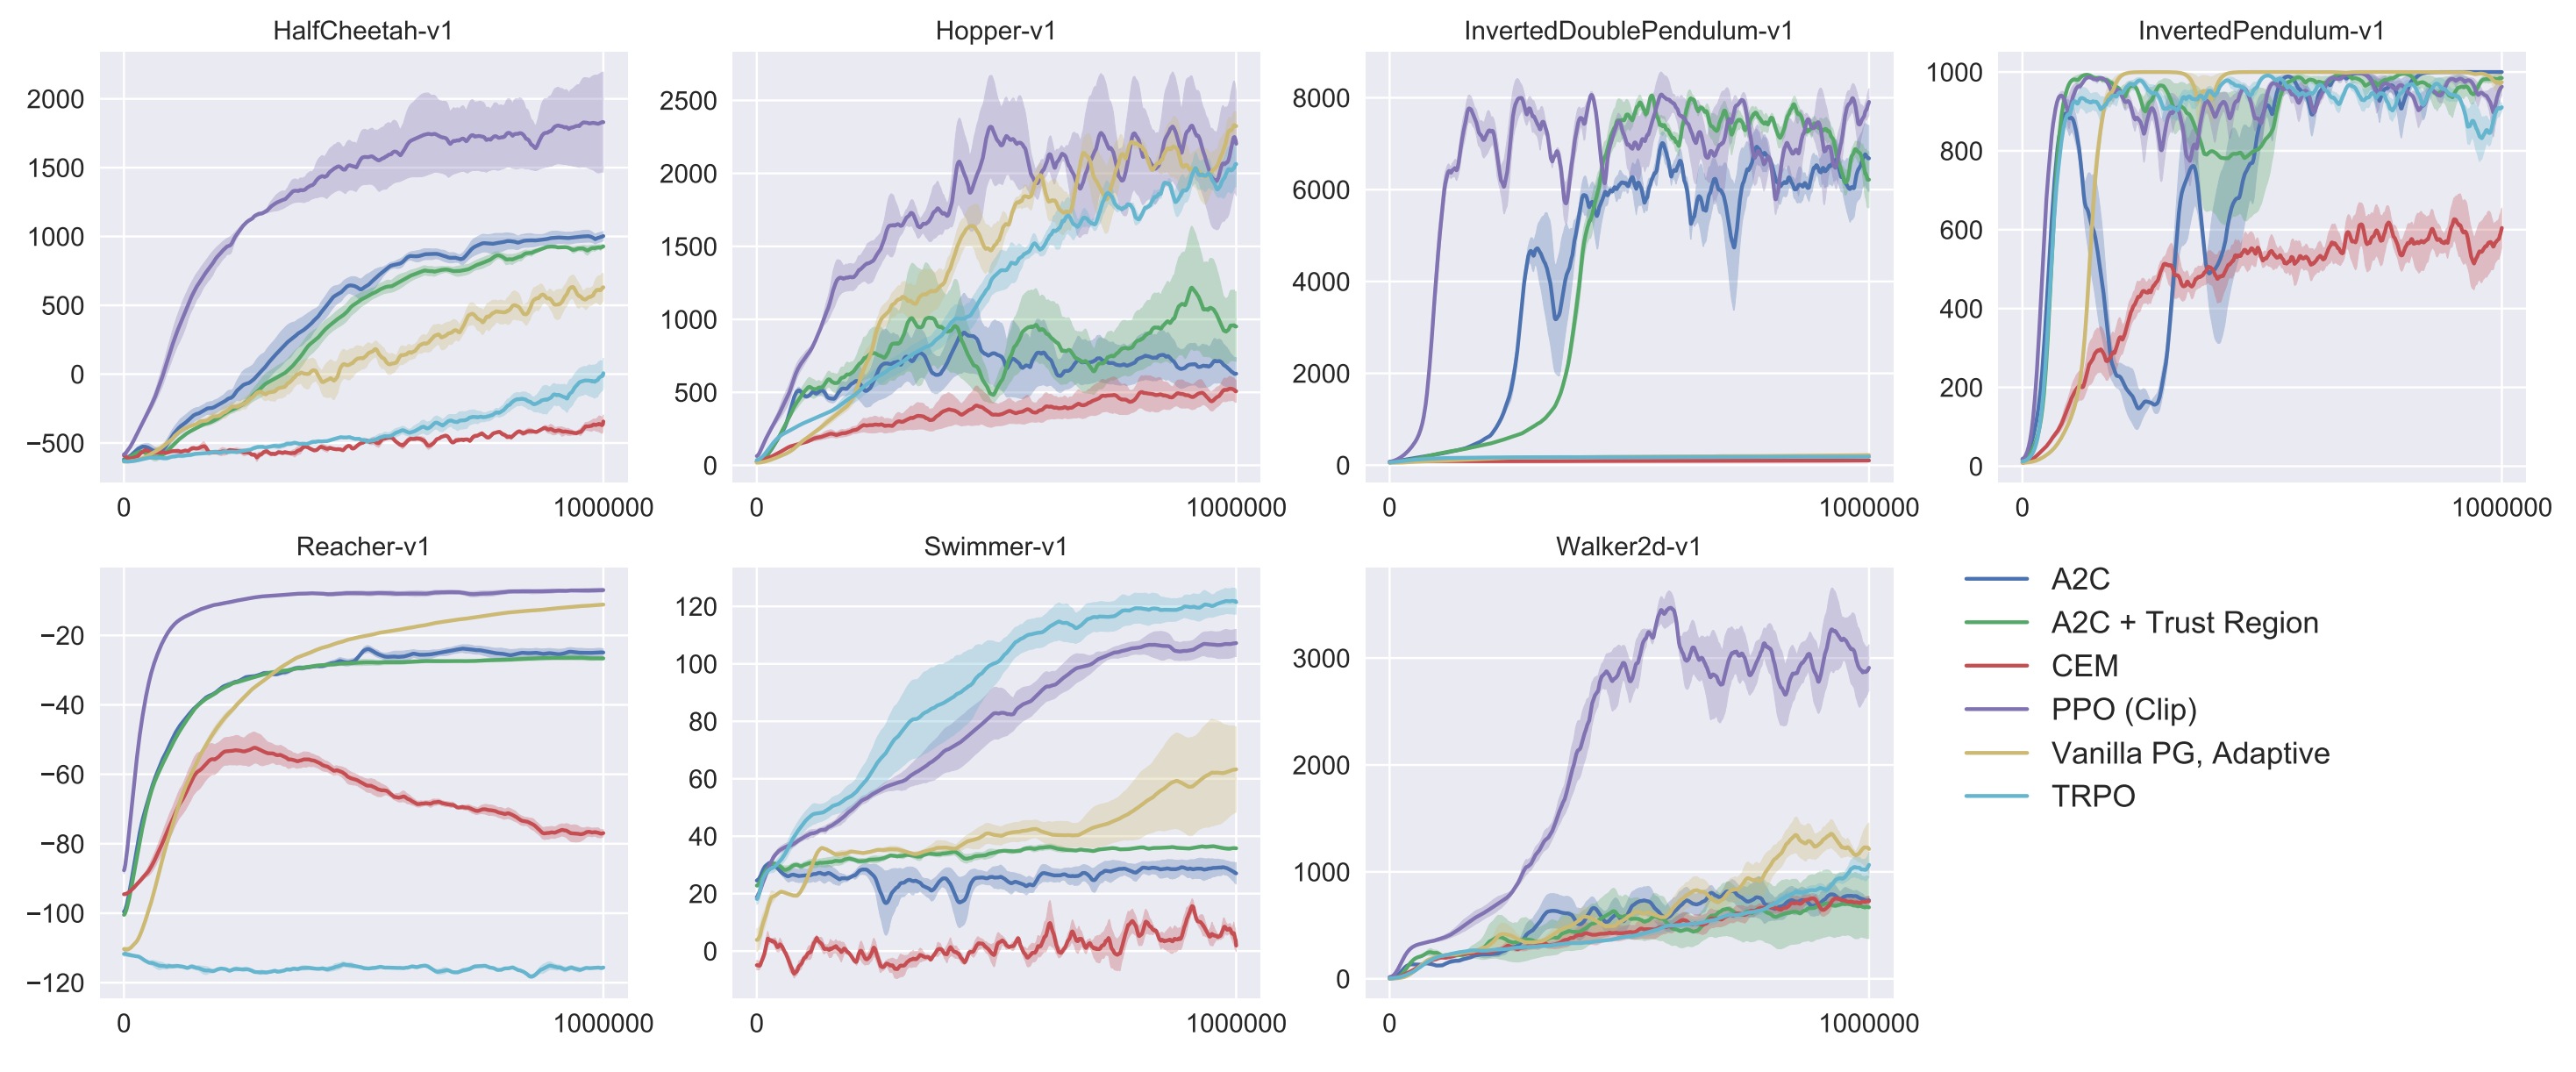
\includegraphics[width=\textwidth]{figures/01/ppo_paper_comparisons.png}
    \caption{Comparison of \ac{ppo} with \ac{trpo} and various other algorithms on several benchmark environments, taken from \cite{ppo}}
    \label{fig:ppo_paper_compare}
\end{figure}


\subsection{Actor Critic Deep Reinforcement Learning}\label{subsec:ac_drl}

With both value-based and policy-based methods introduced, the backdrop is set for actor-critic methods. In both these predecessor methods, either the value-function or the policy is being approximated by a \ac{dnn}, this has a big disadvantage of still being ham-strung by the curse of dimensionality when either action or state space is large. Specifically, value-based methods can perform well when the state space is large and the action space is small, while policy-based methods perform well when the action space is large and the state space is small.


For continuous control problems with continuous state and action spaces, both cases are true. The logical solution is therefore to use function approximators for both value and policy functions, with \ac{dnn} being the popular approximator candidate. This architecture is called \textit{actor-critic}, where the \textit{actor} refers to the policy or the \ac{dnn} approximating the policy, and \textit{critic} refers to the value function or the approximating \ac{dnn}. They can also commonly be referred to as actor/critic networks.

Moreover, because actor-critic method models both value and policy functions, such methods typically involve improving one function after the other. This structure is reminiscent of the generalized policy iteration idea from dynamic programming, mentioned in \autoref{subsec:gpi}, showing that interestingly many ideas within reinforcement learning build upon and are related to one another.

\subsubsection{Deep Deterministic Policy Gradient}

Lillicrap et al. identified many of the same problems stated in this subsection's introduction, and combined the experience replay and target network ideas of \ac{dqn} for value function training, along with the ability of policy-based algorithm to handle continuous action spaces, to build the actor-critic algorithm known as \ac{ddpg} \cite{ddpg}.

The core algorithm of \ac{ddpg} is based on \ac{dpg}, this algorithm is already an actor-critic algorithm but does not use deep neural networks for any function approximation, hence the lack of \textit{deep} in \ac{dpg}. \ac{dpg} uses a deterministic policy as opposed to a stochastic policy, this results in more efficient gradient determinations as the gradient of deterministic policies only requires integrating over the state-space, rather than over the state-\textit{action}-space which is required for gradients of stochastic policies \cite{dpg}. An intuitive explanation behind this difference is that stochastic policies have a non-zero probability of taking each action in the action-space, thus to evaluate the change in optimality of such a policy, it is necessary to consider the entire action space, the same is not true for deterministic policies since they can only take one action for any given state.

\ac{dpg} in it's original form is incompatible with using \ac{dnn} for function approximation, as using such approximations results in the applied gradient computations becoming incorrect estimations of the true policy gradient \cite{dpg}. However, by applying the tricks of experience replay and target networks from \ac{dqn}, \ac{ddpg} is able to extend \ac{dpg} to employ \ac{dnn} for function approximation as well. Specifically, Lilicrap et al. used replay buffers to train their actor and critic networks, in addition to creating target networks for both the critic and actor thus stabilizing learning.

The crux of \ac{ddpg} algorithm is in how it trains the actor and critic. This is done by sampling a minibatch of $N$ transition tuples $(s_i, a_i, s_{i+1}, r_i)$from the replay buffer, and using this minibatch of samples to determine the loss function of \autoref{eq:ddpg_critic_loss} which the critic is trained to minimize, and the policy gradient \autoref{eq:ddpg_policy_gradient} used to update the actor.

{\myfont
\begin{align*}
    J_c &= \frac{1}{N}\sum\limits_i (y_i - Q(s_i, a_i, \boldsymbol{\theta}_c))^2  \stepcounter{equation}\tag{\theequation}\label{eq:ddpg_critic_loss}\\
    y_i &= r_i + \gamma Q(s_i, \pi(s_{i+1}, \boldsymbol{\theta}^T_a), \boldsymbol{\theta}^T_c) \stepcounter{equation}\tag{\theequation}\label{eq:y_i_ddpg}\\
    \nabla_{\boldsymbol{\theta}_a} J_a &= \frac{1}{N}\sum\limits_i \nabla_a Q\big(s_i,\pi(s_i, \boldsymbol{\theta}_a),\boldsymbol{\theta}_c\big) \nabla_{\boldsymbol{\theta}_a} \pi(s_i, \boldsymbol{\theta}_a) \stepcounter{equation}\tag{\theequation}\label{eq:ddpg_policy_gradient} \\
    \text{Where } \quad \boldsymbol{\theta}^T &= \text{ target network parameters}
\end{align*}
}

A noteworthy achievement of the \ac{ddpg} algorithm is its ability to triumph in the face of the deadly triad; \ac{ddpg} uses function approximations, it updates the critic network through a \ac{td} like method, and it is an off-policy method due to using experience replay for training. Demonstrating superior performance than \ac{dpg} on which it was based \cite{ddpg}.


\subsubsection{Twin Delayed DDPG}

One problem with \ac{ddpg} is shown to be inherited from value-based methods by Fujimoto et al., and this is the over-optimism of value function estimates in the critic network. Within the realm of value-based research, this issue has already been addressed through the introduction of double learning by van Hasselt \cite{double_q_learning}, with duplicate value networks. This is not to be confused with the duplicate networks of the target-network solution which deliberately slows down training of the target network, while double training randomly selects one of the duplicate networks for training. 

Fujimoto et al. thus introduced double learning to \ac{ddpg} by training two critic networks at the same time, resulting in the \ac{td3} algorithm. In addition to using double learning, \ac{td3} also improved over \ac{ddpg} in two more ways. Firstly, the updates to the actor and critic are made asynchronous, with the value estimates of the critic being updated at a higher rate than the actor's policy, which mitigated the occurrence of divergent updates to policy parameters and constitutes the \textit{delayed} part in the name of \ac{td3}. 

The second improvement is to add a bit of noise to the critic learning. In \ac{ddpg} the critic is trained using a \ac{td} learning approach with a learning target being obtained using the deterministic actor, introducing this determinism into the learning target can cause value-learning to suffer from high variance. Thus to combat this variance, the learning target for the critic is instead not picked using only the deterministic action from the actor, but with some noise added to the action before the learning target is retrieved from the critic. Which can be done by changing the formulation of \autoref{eq:y_i_ddpg} to add some clipped random variable $\epsilon$, which for example can be distributed normally $\epsilon \sim clip(\mathcal{N}(0, 0.1), -c, c)$, resulting in the reformulated learning target $y_i$ being:

\begin{equation}
    y_i = r_i + \gamma Q\big(s_i, \pi(s_{i+1}, \boldsymbol{\theta}^T_a) + \epsilon, \boldsymbol{\theta}^T_c\big)
\end{equation}

\subsubsection{Soft Actor Critic}

Around the same time but independent of the efforts of Fujimoto et al., Haarnoja et al. \cite{sac} posed an alternative set of improvements to \ac{ddpg} which culminated in the \ac{sac} algorithm. 

As opposed to the algorithms discussed thus far, \ac{sac} uses the unique goal maximizing return and randomness simultaneously, which is an approach called \textit{maximum entropy reinforcement learning} \cite{maximum_entropy}. In this framework, the optimality of a policy is measured not solely by the expected return, but by an expectation over the sum of return and entropy:

{\myfont
\begin{equation}
    J(\pi) = \sum\limits_t \mathbb{E}[r_t + \parunderbrace{\alpha \mathcal{H}(\pi(s_t))}{entropy of policy}]
\end{equation}
}

Where $\alpha$ is a temperature parameter that weighs how important being random is, and the entropy function $\mathcal{H}$ measures how random a policy is. Formulating such a loss function leads to the agent seeking to learn the most rewarding policy which is also most stochastic, Such a policy is crucial in the early stages of training, as it allows an agent to explore state and actions more widely thanks to the loss function favouring random actions, which can increase the odds of finding a near-globally optimal policy. Logically, if a deterministic policy was used, then this improvement would not have contributed to any changes in the algorithm's behaviour. Thus, Haarnoja et al. returned to using stochastic policies for the actor-network, in \ac{sac} the policy is modelled as a multivariate but diagonal Gaussian, with the actor-network outputs being the Gaussian's mean and covariance.

In addition to adopting a maximum entropy framework to evaluate its policy, \ac{sac} also uses several of the improvements present in \ac{td3}. This includes the double action-value learning trick introduced by van Hasselt \cite{double_q_learning}, where just like in \ac{td3} two action values are trained simultaneously, and a less optimistic value estimate is taken by sampling the minimum action value from the two critics when calculating the learning target for a given state-action pair. 

% \subsection{General Intelligence DRL}

% The biggest reason why \ac{drl} as a field is the most exciting amongst all the artificial intelligence fields is its combination of two important machine learning paradigms into one; that of deep learning which allows patterns and information to be ascertained from extremely high dimensional input data formats such as video and audio streams, and that of reinforcement learning which allows a machine to replicate biological learning in animals. To move this field further in biological imitation, the architecture of reinforcement learning algorithms is continuously innovated to allow agents to learn in more and more complex manners.

% One way in which this is done is in the framework of \textit{hierarchical reinforcement learning}. This framework seeks to improve the sample efficiency of so-called \textit{flat reinforcement learning} methods, which are methods referred to by Dietterich \cite{hrl_dietter} with only one layer of policies and value functions, the case of all algorithms described thus far. In the hierarchical framework, the goal is to decompose a given \ac{mdp} into smaller processes and train the agent on each of them, an approach analogous to dynamic programming in the sense of decomposing and solving subproblems. This decomposition allows for the opportunity of \textit{state abstractions}, where states that belong to the same processes can be grouped together, and an agent can focus on one group of sets for training at one time, or train for different groups of states and processes in parallel \cite{hrl_dietter}. Another pillar of the hierarchical framework is \textit{temporal abstraction}, which is when states or actions are modelled as extending over multiple time steps. When an action spans over some time, it is referred to as an \textit{option} \cite{hrl_ron, hrl_dietter}.

% These and various other disparate ideas from the hierarchical framework are recapitulated by Barreto et al. into the \textit{options keyboard}, which provides the mechanisms necessary to create self-learning agents that can navigate complex environments where multiple types of tasks and rewards exist \cite{options_keyboard}.


\section{Flying-V}
The Flying-V is a novel design for jet-powered passenger airliners, it features a distinct V-shaped flying wing body which contains the passenger and cargo compartments while promising the potential for more sustainable aviation through efficient flight \cite{benad2015flying, benad2022design}. This aircraft design will serve as the environment in the \ac{mdp} that the developed reinforcement learning agent will control, and thus this section will serve to introduce the background on this aircraft and relevant notes of the design.

This section will begin with an overview of the Flying-V design and overall characteristics in \autoref{subsec:v_overview}...

\subsection{Flying-V Overview}\label{subsec:v_overview}

The design of this aircraft focused on improving the efficiency of commercial jet airliners, which have a tube and wing configuration and present additional undesired parasitic drag from the tube fuselage. At cruising altitude, passenger cabins are pressurized to provide comfortable breathing conditions, consequently, passenger cabins are shaped like a cylinder as it is a structurally efficient geometry for pressurized vessels. By placing the passenger cabins along the span of a heavily swept-back wing, it is possible to use a cylindrical shape to retain this structural efficiency, in addition to more efficiently fitting the cabin inside an airfoil profile and thus reducing the cabin's parasitic drag. This serves as the primary design factor driving the design of the Flying V, resulting in the $\Lambda$ shape of this aircraft's design \cite{benad2015flying}, depicted in \autoref{fig:flying_v_1}.

\begin{figure}[h]
    \centering
    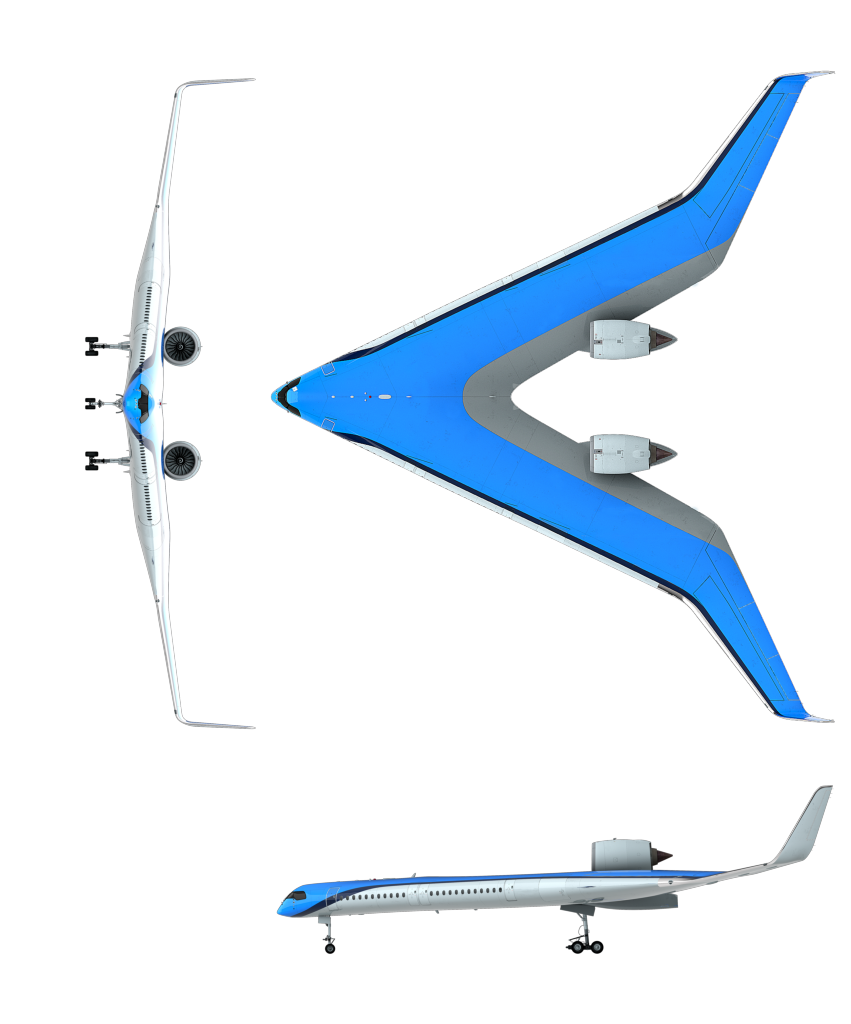
\includegraphics[width=0.6\textwidth]{figures/01/v_3.pdf}
    \caption{}
    \caption[notsure what this for]%
    {Artist's impression of the Flying V\footnotemark.}
    \label{fig:flying_v_1}
\end{figure}

\footnotetext{Retrieved from \url{https://www.tudelft.nl/en/ae/flying-v}}

This configuration results in both aerodynamic and structural efficiency improvements when compared to the A350-900, which is in the same category of passenger capacity and flight range. Aerodynamically, the Flying-V has demonstrated a 10-\% higher lift-to-drag ratio than the A350 \cite{benad2015flying}, which allows it to carry more payload for the same extent of drag and thus ferry passengers more efficiently. Moreover, it has an estimated structural weight saving of 17\% compared to an A350-like design \cite{claeys2018flying, van2017development}, not only making it more material-efficient but also requiring less lift to fly. Unlike contemporary airliners, the engine of the Flying-V is placed above the wings, which will shield the noise generated by the turbofan engines from the ground, and is expected to reduce noise pollution, especially during the terminal flight phases of takeoff and landing. 

The Flying-V is a design which is being actively improved upon. Using a 4.6\%-scale model of the aircraft for wind tunnel tests, Palermo and Vos experimentally deduced an optimal range of location to place the design's center of gravity to ensure longitudinal stability \cite{palermo2020experimental}, which served as an important variable to base future design work upon. Engine positioning as well as its effect on the aerodynamics of the Flying-V were investigated through numerical simulations by Pascual and Vos \cite{rubio2020effect}, who noted the extreme detrimental impact of misplacing the engines which at worst resulted in a lift-to-drag ratio loss of 55\%, and selected a position which compromised between minimal aerodynamic efficiency loss and controllability under a one-engine inoperative scenario. The aerodynamic effects of this engine placement was further investigated experimentally in a wind tunnel using the 4.6\%-scale model by van Empelen and Vos \cite{van2017development}, who showed that the engine installation resulted in a small increase of the lift-curve slope, and found an upper bound for the nose-down moment cause by engine thrust. The concept was then extended to a family of designs by Oosterom and Vos \cite{oosterom2022conceptual}, who presented a three-member \textbf{FV-XXX} family concept, key characteristics of each member in the family are tabulated in \autoref{tab:v_family}.

\begin{table}[h]
    \centering
    \caption[test]{Flying-V family of designs\cite{v_design}.}
    \label{tab:v_family}
    \begin{tabular}{|L{3cm}|L{1.6cm}|L{1.1cm}|L{1.1cm}|L{1.1cm}|}
    \hline
    \rowcolor{Bluetab}
         \multicolumn{1}{|c}{\textbf{Parameter}} & \multicolumn{1}{|c}{\textbf{Unit}} & \multicolumn{1}{|c|}{\textbf{FV-800}} & \multicolumn{1}{|c|}{\textbf{FV-900}} & \multicolumn{1}{|c|}{\textbf{FV-1000}} \\ \hline
         Wing span       & [$m$]            & 55.5   & 60.7  & 65    \\ \hline
         Passengers      & [-]              & 293    & 328   & 361   \\ \hline
         Design range    & [$km$]           & 11,200 & 14800 & 15300 \\ \hline
         OEW             & [$kg\times10^3$] & 99.9   & 115   & 129   \\ \hline
         MTOW            & [$kg\times10^3$] & 185    & 234   & 266   \\ \hline
    \end{tabular}
\end{table}

The outboard wing geometry was optimized under a study by van Luijk and Vos \cite{van2023constrained}, this optimization was performed with constraints on the area, wing planform limits, and the integration of elevon surfaces. This geometry optimization resulted in a wing design that increased the lift-to-drag ratio of the Flying-V by a further 8.4\%.

\subsection{Flight Control Challenges}\label{subsec:v_challenges}

The traditional tube-and-wing design of an aircraft has been widely adopted due to its inherently stable and easy to trim nature. The location of horzontal and vertical stabilizers all the way at the tail end of an aircraft allows these surfaces to provide a high degree of passive stabilizing moments, resulting in the yawing and pitching moment coefficients of such designs to reach stabilizing values easily. Their effects can be compared to that of the fins at the tail end of an arrow, which places the center of pressure aft of the center of gravity, which allows the aerodynamic forces to naturally steer the arrow into a straight flight.

In a flying wing design such as the Flying-V, this natural stability is largely forgone. Instead, the sweep of the wings needs to be sufficiently high in order to recoperate these lost stabilizing moments. Despite such design compensations, stable flight in flying wing and blended wing body designs can be difficult, due to reasons of limited moment arms reducing control effectiveness \cite{bad_moment_arm}, strong coupling in the dynamics leading to nonlinear control effects \cite{bad_coupling}, and the propensity for sudden pitch up behaviour at high angles of attack \cite{flying_wing_bad_1}.

Regarding the flight dynamics of the Flying-V specifically, cappuyns \cite{cappuyns2019handling} performed numerical simulations of the design using a vortex lattice method, and observed that the handing qualities for some eigenmodes are slightly subpar, such as the dutch roll mode during cruise, which is in fact slightly unstable as it has a negative damping factor. This observation was separately found by van Overeem et al. \cite{overeem_modelling}, who performed numerical studies of the Flying-V using mathematical models built from wind tunnel data, found that overall the handling qualities of the Flying-V were sub-par, and also observed that the dutch roll mode was slightly unstable during cruise. During approach, van Overeem et al. saw that additional eigenmodes became unstable, namely the phugoid, spiral, and short period modes.

\subsection{Flying-V Control System}\label{subsec:v_fcs}

For a flight controller, the most important design aspects of the Flying-V is the layout of it's flight control system, specifically the control surfaces available and their control effectiveness. As the Flying-V does not have a tail like in traditional aircraft designs, the flight control surfaces that are traditionally located on the horizontal and vertical stabilizers of the empennage are moved to the main wing. This results in a control surface layout which features rudder surfaces on the vertical winglets providing control moments for yawing, and a series of control surfaces referred to as \textit{elevons} along the trailing edge of the wing tip, which combines the functionalities of elevator and aileron providing control moments for rolling and pitching. Along the development history of the Flying-V, three main layouts for its flight control surfaces have been identified. While all three layouts used consistent rudder designs, they differed in how the elvons were configured:

\begin{enumerate}
    \item Configuration adopted by Palermo \cite{palermo2019longitudinal}, Palermo and Vos \cite{palermo2020experimental}, and Garcia et al. \cite{ruiz2020aerodynamic} split the elevon into 3, an inner-board elevon CS1 used for pitch control, a mid-board elevon CS2 used for pitch and roll control, and an out-board elevon CS3 used for roll control.
    \item Configuration adopted by Nolet \cite{split_flap_nolet} which also split the elevons into 3, but added a split flap surface out-board from CS3 elevons to provide additional yaw control and combating directional instability.    
    \item Configuration adopted by Cappuyns \cite{cappuyns2019handling} split the elevons into 2, an inner-board elevon CS1 and an outer-board elevon CS2 used for pitch and roll control respectively.
\end{enumerate}

\begin{figure}[h]
     \centering
     \begin{subfigure}[b]{0.3\textwidth}
         \centering
         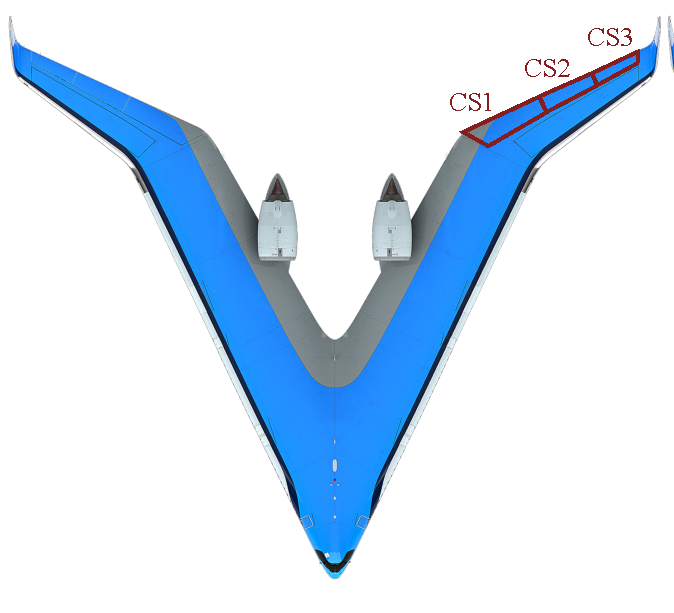
\includegraphics[width=\textwidth]{figures/01/3_elevons.png}
         \caption{3 elevons configuration \cite{palermo2020experimental}}
         \label{subfig:3_elevons}
     \end{subfigure}
     \hfill
     \begin{subfigure}[b]{0.3\textwidth}
         \centering
         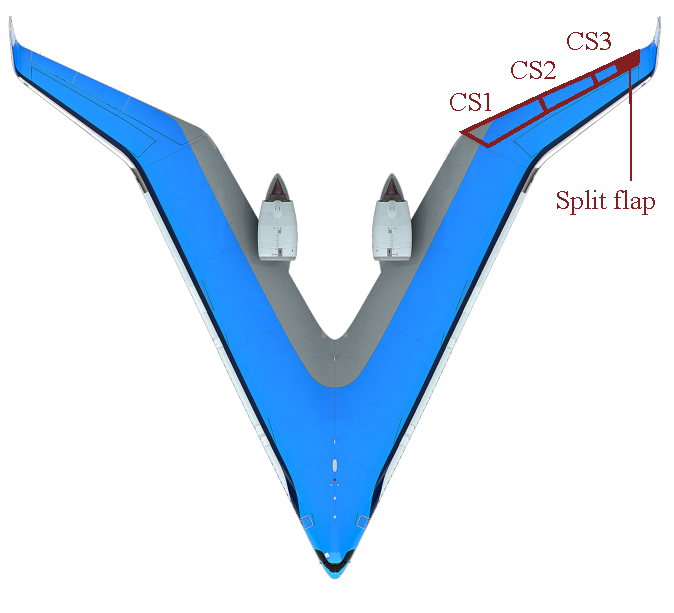
\includegraphics[width=\textwidth]{figures/01/3_elevons_split_flap.png}
         \caption{3 elevons plus split flaps configuration \cite{split_flap_nolet}}
         \label{subfig:3_elevons_split_flap}
     \end{subfigure}
     \hfill
     \begin{subfigure}[b]{0.3\textwidth}
         \centering
         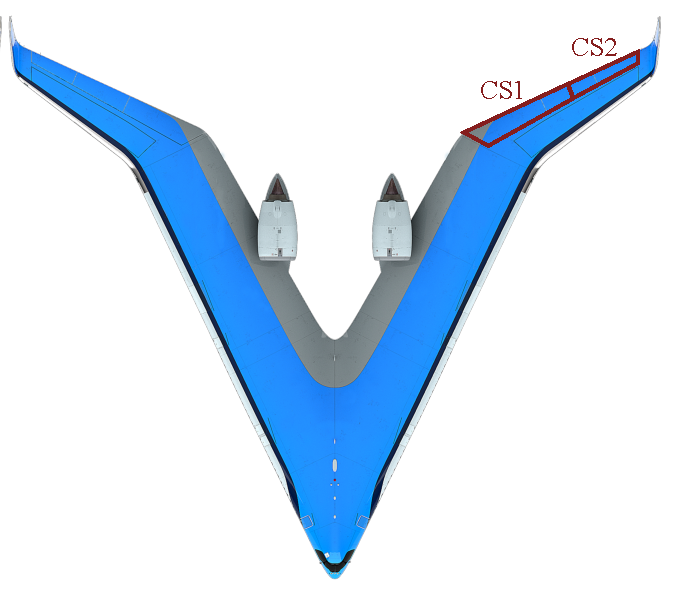
\includegraphics[width=\textwidth]{figures/01/2_elevons.png}
         \caption{2 elevons configuration \cite{overeem_modelling}.}
         \label{subfig:2_elevons}
     \end{subfigure}
        \caption{The various control surface setups used in various research efforts.}
        \label{fig:3_setups}
\end{figure}
\subsection{Dynamics Modelling}\label{subsec:v_model}

To b

\section{Flight Control by Reinforcement Learning}\label{sec:rl_flight_control}

In recent years, various deep reinforcement learning algorithms have been applied to the task of flight control. These algorithms have been used to train flight controllers for a number of aircraft types, including fixed-wing aircraft, quadcopters, and helicopters. 


\subsection{Flight Control as an MDP}\label{subsec:flight_control_mdp}

The goal of this thesis is to develop an intelligent flight control system for the Flying-V, thus it is important to understand how the flight control problem is formulated, and how that can be translated into a problem that a reinforcement learning agent can handle. 

\subsubsection{Formulating the MDP}

The flight control environment is constituted of two components: the flight dynamics, and the reference trajectory. The flight dynamics component receives the action from the agent and computes how the aircraft states evolved, and then the target state that the aircraft should have is obtained from the reference trajectory. To arrive at the states and rewards of the \ac{mdp}, this target and actual state are combined to produce the process's states and rewards. The specific way in which they are combined depends on the design of the \ac{mdp}. 

As an example, in Dally and van Kampen's work \cite{killian}, the states $\bold{x}$ of the aircraft are shown in \autoref{eq:killian_ac_states}, and the reference trajectory adopted defines targets for the sideslip, pitch, and roll states, as shown in \autoref{eq:killian_ref_states}. In this work, two reinforcement learning controllers are implemented, meaning there are two \ac{mdp}s to be defined here, for simplicity's sake this explanation will concern itself with only one controller: the attitude controller. To define the \ac{mdp} states for this agent, the aircraft states $\bold{x}$ and reference trajectory $\bold{x}_{ref}$ are first combined to produce an error vector $\bold{e}$, defined in \autoref{eq:killian_err_vec}. This error vector is then weighted producing $\bold{e}_w$, and concatenated with the aircraft's current control surface deflections and aircraft attitude rates, to produce the \ac{mdp} states $\bold{s}$ shown in \autoref{eq:killian_mdp_states}. The inclusion of the control surface deflections may seem redundant, however, it was necessary in the case of this controller due to the agent only providing \textit{increments} to the control surface deflections; thus providing the agent with knowledge of what current deflections are, gave more context on what increments should be fed back to the aircraft. The reward $r$ of this \ac{mdp} is then created by using $\bold{e}_w$, which is clipped to $[-1, 0]$, the norm of it taken and scaled, as shown in \autoref{eq:killian_mdp_reward}.

{\myfont
\begin{align*}
    \bold{x} &= \begin{bmatrix} p & q & r & V & \alpha & \beta & \theta & \phi & \psi & h \end{bmatrix}^{\top} \stepcounter{equation}\tag{\theequation}\label{eq:killian_ac_states} \\
    \bold{x}_{ref} &= \begin{bmatrix} \beta_{ref} & \theta_{ref} & \psi_{ref} \end{bmatrix}^{\top} \stepcounter{equation}\tag{\theequation}\label{eq:killian_ref_states} \\
    \bold{e} &= \begin{bmatrix} \beta_{ref} - \beta & \theta_{ref} - \theta & \psi_{ref} - \psi \end{bmatrix}^{\top} \stepcounter{equation}\tag{\theequation}\label{eq:killian_err_vec} \\
    \bold{s} &= \begin{bmatrix} \bold{e}_{w}^{\top} & \delta_a & \delta_e & \delta_r & p & q & r\end{bmatrix}^{\top} \stepcounter{equation}\tag{\theequation}\label{eq:killian_mdp_states} \\
    r &= -\frac{1}{3}\| \text{clip}(\bold{e}_w, -1, 0) \| \stepcounter{equation}\tag{\theequation}\label{eq:killian_mdp_reward} \\
\end{align*}
}

\subsubsection{Modelling Flight Dynamics}


A flight dynamics model in its general form is modelled as two systems of ordinary differential equations which are functions of a vector of states $x$ and a vector of inputs $u$. The first system models the derivative of the states $\dot{\bold{x}}$ at any given time for the given state and inputs using the state transition functions $f(\cdot)$, whereas the second system models observations $\bold{y}$ using the observation equations $g(\cdot)$, which is how states are observed from the aircraft in a real-life system where the states are not necessarily directly known. Such a representation is shown in \autoref{eq:nonlin_ss}

\begin{align*}
    \dot{\bold{x}} &= f(\bold{x, u}) \stepcounter{equation}\tag{\theequation}\label{eq:nonlin_ss}\\
    \bold{y} &= g(\bold{x, u}) 
\end{align*}

These differential equations describe the motion of an aircraft in three-dimensional continuous space, but the motion has six degrees of freedom where three degrees belong to the translational motions and the remainder for rotational motions. The states of these equations typically consist of the aircraft's position $\bold{p}$, velocity $\bold{v}$, attitude $\bold{a}$, and attitude rates $\boldsymbol{\Omega}$:
{\myfont
\begin{align*}
    \bold{x} &= \begin{bmatrix}
        \bold{p} & \bold{v} & \bold{a} & \boldsymbol{\Omega}
    \end{bmatrix}^T \\
    \text{Where } \quad \bold{p} = \begin{bmatrix} x & y & z\end{bmatrix}^{\top} \quad \bold{v} &= \begin{bmatrix}u & v & w \end{bmatrix}^{\top} \quad \bold{a} = \begin{bmatrix} \phi & \theta & \psi \end{bmatrix}^{\top} \quad \boldsymbol{\Omega} = \begin{bmatrix}p & q & r \end{bmatrix}^{\top}
\end{align*}
}

The inputs vector $\bold{u}$ typically consists of the control surface deflections $\delta_a, \delta_e, \delta_r$, thrust settings $T$. They are typically bounded by physical limits, which are referred to as saturation limits:
{\myfont
\begin{align*}
    &\bold{u} = \begin{bmatrix}
        \delta_a & \delta_e & \delta_r & T
    \end{bmatrix}^{\top} \\
    \text{Subject to } \quad &\bold{u}_{min} \leq \bold{u} \leq \bold{u}_{max}
\end{align*}
}

This way of modelling system dynamics is called a \textit{state-space} representation, which is signified by the use of first-order differential equations to model the evolution of states over time. The state-space representation of an aircraft can be formulated using nonlinear dynamics, which is implied when the state transition functions are denoted using lowercase $f$ and are a function of states and/or inputs. It can also be modelled using fully linear dynamics, which is referred to as a \ac{lti} model when the model parameters stay fixed over time, where the system is denoted in the following manner:

\begin{align*}
    \dot{\bold{x}} &= \bold{Ax} + \bold{Bu} \stepcounter{equation}\tag{\theequation}\label{eq:lin_ss}\\
    \bold{y} &= \bold{Cx} + \bold{Du} 
\end{align*}

Where $\bold{A, B, C, D}$ are referred to as the state transition matrix, the input matrix, the output matrix, and the feedforward matrix respectively. \ac{lti} serves as a very useful tool, as it allows for many standard flight control design and evaluation practices to be employed. For example, they allow robust control techniques to be readily applied as the theory of $\mathcal{H}_{\infty}$ synthesis is founded on theory applicable only to linear systems, they allow for feedback gains to be readily calculated and thus for feedback controllers to be quickly developed, and they allow for the stability of the aircraft to be quickly analyzed by simple computation of the eigenvalues of the system \cite{skogestad}. A time-varying version of the linear state-space model is used in the incremental \ac{acd} case, where the $\bold{A, B}$ matrices would have different parameters over time.

To make these models useful for computing the states of the aircraft needed for an \ac{mdp}, system state derivatives are integrated to compute the states in the next time step. This procedure can be simplified and a discrete version of \autoref{eq:nonlin_ss} obtained, defining the states and observations of the next time step:


\begin{align*}
    \bold{x}_{t+1} &= f(\bold{x_t, u_t}) \stepcounter{equation}\tag{\theequation}\label{eq:discrete_ss}\\
    \bold{y}_t &= g(\bold{x_t, u_t}) 
\end{align*}

Finally, the deterministic form shown in \autoref{eq:discrete_ss} is Markovian, as the states and inputs from the current timestep $t$ are enough to predict the states and observations for the next timestep $t+1$. The Markovian property remains even when stochasticity is introduced as long as no time correlation is present in this noise, methods do nonetheless exist that allow pseudo-time-correlated noise to be introduced to the model while remaining Markovian \cite{stochastic_forcing}.


\subsection{Learning to Fly}\label{subsec:learning_to_fly}

Flight control poses a formidable environment for reinforcement learning agents to excel in. The level of difficulty varies between aircraft designs, in agile aircraft such as fighter planes, the dynamics of such vehicles are highly unstable \cite{unstable_1, unstable_2, unstable_3} in order to perform fast manoeuvres for the least amount of input, but as a result can easily succumb to catastrophic loss of control. In contrast, commercial airliners are designed to be stable and easy to control \cite{stable_1, stable_2}, and thus offer a less harsh learning environment for an agent. Additionally, the coupled nature between control actions in one axis and state changes in a separate axis makes the control problem a high-dimensional and non-linear one, which adds to the challenge for reinforcement learning agents to learn to control an aircraft.

\subsubsection{Past Research in RL for Flight Control}

One of the earliest works to apply reinforcement learning to flight control was by Abbeel et al. \cite{abbeel2006application}, who formulated an LQR problem for the task of acrobatic helicopter flights and used a specific instance of reinforcement learning named differential dynamic programming to solve for the posed LQR's optimal policy. The result was a controller which can perform acrobatic manoeuvres such as flips and rolls, manoeuvres that are challenging even for human pilots. 

\ac{ddpg} appears to be a popular \ac{drl} algorithm applied to flight control. Fei et al. \cite{flappy_bird}managed to apply \ac{ddpg}, specifically a benchmark implementation by Duan et al. \cite{benchmark_drl_algos}\footnote{Implementations available at \url{https://github.com/rlworkgroup/garage}}, to the flight control of a flapping wing robot. This \ac{ddpg} agent was trained to copy the extreme manoeuvre which hummingbirds can execute during fast escapes and managed to replicate the manoeuvre. \ac{ddpg} was also adopted by De Marco et al. \cite{de2023deep} in their research into flight control for an F-16 in a flight simulation, here the agent is trained to successfully fly an F-16 in a sequence of agile turns and manoeuvres with highly coupled dynamics, under the presence of sensor noise. The trained agent was duplicated and placed in a simulation of a prey-chaser scenario, where a prey agent was given a sequence of waypoints to follow, and a chaser agent was given the task of catching up to the prey, showing an interesting case of multi-agent interaction. This algorithm was also applied to the autonomous landing of fixed-wing aircraft in \cite{ddpg_landing} and longitudinal control augmentation in \cite{ddpg_lcas}.

A different \ac{drl} algorithm that has demonstrated success in flight control is the \ac{sac} algorithm. Where Dally and van Kampen developed a flight controller for a Cessna Citation 500 aircraft trained using \ac{sac}, alluded to in \autoref{subsec:flight_control_mdp}. The control structure used in this research was cascaded, while the overall controller controlled the aircraft's altitude, roll, and sideslip angle, the task was delegated to an inner and outer controller. The outer \ac{sac} controller handled altitude control by taking in reference altitude and providing a reference pitch angle for the subsequent inner \ac{sac} controller, which handled attitude control by taking in the reference pitch, roll, and sideslip, and providing control surface deflection increment commands to the aircraft. The \ac{sac} controller proved to be robust and fault-tolerant, wherein it remained performant in the face of various disturbances, control system failures, and fault scenarios.


% hummingbird ran for 500 episodes (500k transitions)
% high perf ran for 2900 episodes (200k transitions), converged in 500 episodes (30k transitions)

First talk about the deep learning based flight controllers, then go to Casper's work which directly compares \ac{drl} with adp work, and use this to segue over to adp applications to flight control.

Evolution of IDHP-based controller:

\begin{itemize}
    \item Ye Zhou: IDHP for pitch control, using nonlinear short-period missile model.
    \item Stefan Heyer: PID for outer slow dynamics control (altitude, roll, sideslip), IDHP with target network for slower and stable inner loop fast dynamics control (roll, pitch, yaw rates), using full 6-DOF citation simulator without yaw damper and with auto-throttle.
    \item JunHyeon Lee: IDHP for slow and fast dynamics control (altitude and pitch angle), using full 6-DOF Ciation simulator with yaw damper and auto-throttle.
    \item Casper: SAC for outer slow dynamics control (altitude), IDHP with SAC pre-trained actor for inner faster dynamics control (roll pitch yaw \textbf{angles}), using full 6-DOF Citation simulator with yaw damper and auto-throttle.
\end{itemize}




cool sources to cite for how advanced DRL can be
\cite{drl_benchmarking, drl_atari, drl_humanlvl}

\section{Synopsis}

% Basic temporal difference algorithms utilize tabular look ups to retreive the value function of each state or state-action pair, this can hinder scaling to larger problem spaces which have many state or action variables, as the number of values to be stored increases combinatorially. The idea was thus put forth that function approximators should be used to approximate these look up tables which provided the scaling power necessary for higher dimensional tasks \cite{function_approximators}, with deep neural networks and multi layer perceptrons becoming popular approximators as they demonstrate a better scalability and approximation power \cite{drl_benchmarking, drl_atari, drl_humanlvl}. However, these function approximators need not necessarily be deep neural networks; in fact, early works focused on the application of simpler and smaller-scale approximations. Such as using coarse tile encoding, linear polynomials, Fourier basis, and many more \cite{intro_rl}.

\end{document}